Este apêndice tem o intuito de expor os resultados obtidos por testes de validação do modelo proposto. Esses testes foram realizados conforme detalhado nos casos de teste, apresentados no \appendixautorefname~\ref{appendix-casosTeste}.

\section{Caso de Teste CT01 Referente a RFS01}
O caso de teste CT01 visou validar se o robô é capaz de se mover para todos os sentidos e direções pelo ambiente que está inserido. O caso de teste foi repetido cinco vezes com o robô em lugares distintos no ambiente. Entre os cinco testes, apenas um foi mal sucedido, visto que o robô rotacionou para o lado errado ao adicionar os obstáculos. Todos os resultados podem ser visualizados na Tabela~\ref{tab:acertosct01}. Além disso, a seguir podem ser encontradas as capturas para cada repetição (Figura~\ref{fig:ct01_1}, Figura~\ref{fig:ct01_2}, Figura~\ref{fig:ct01_3}, Figura~\ref{fig:ct01_4}, Figura~\ref{fig:ct01_5}).

\begin{table}[H]
\centering
\caption{Resultados das repetições CT01}
\label{tab:acertosct01}
\resizebox{\textwidth}{!}{%
\begin{tabular}{l|c}
                              & \multicolumn{1}{l}{\textbf{Resultados CT01}} \\ \hline
\textbf{Teste 1}              & Bem-sucedido                                 \\
\textbf{Teste 2}              & Bem-sucedido                                 \\
\textbf{Teste 3}              & Bem-sucedido                                 \\
\textbf{Teste 4}              & Mal-sucedido                                 \\
\textbf{Teste 5}              & Bem-sucedido                                 \\
\textbf{Total de acertos (\%)} & \textbf{80}                                  \\ \hline
\end{tabular}%
}
\caption*{Fonte: Autora (2023).}
\end{table}

\begin{figure}[H]
    \centering
    \caption{Captura da primeira repetição CT01}
    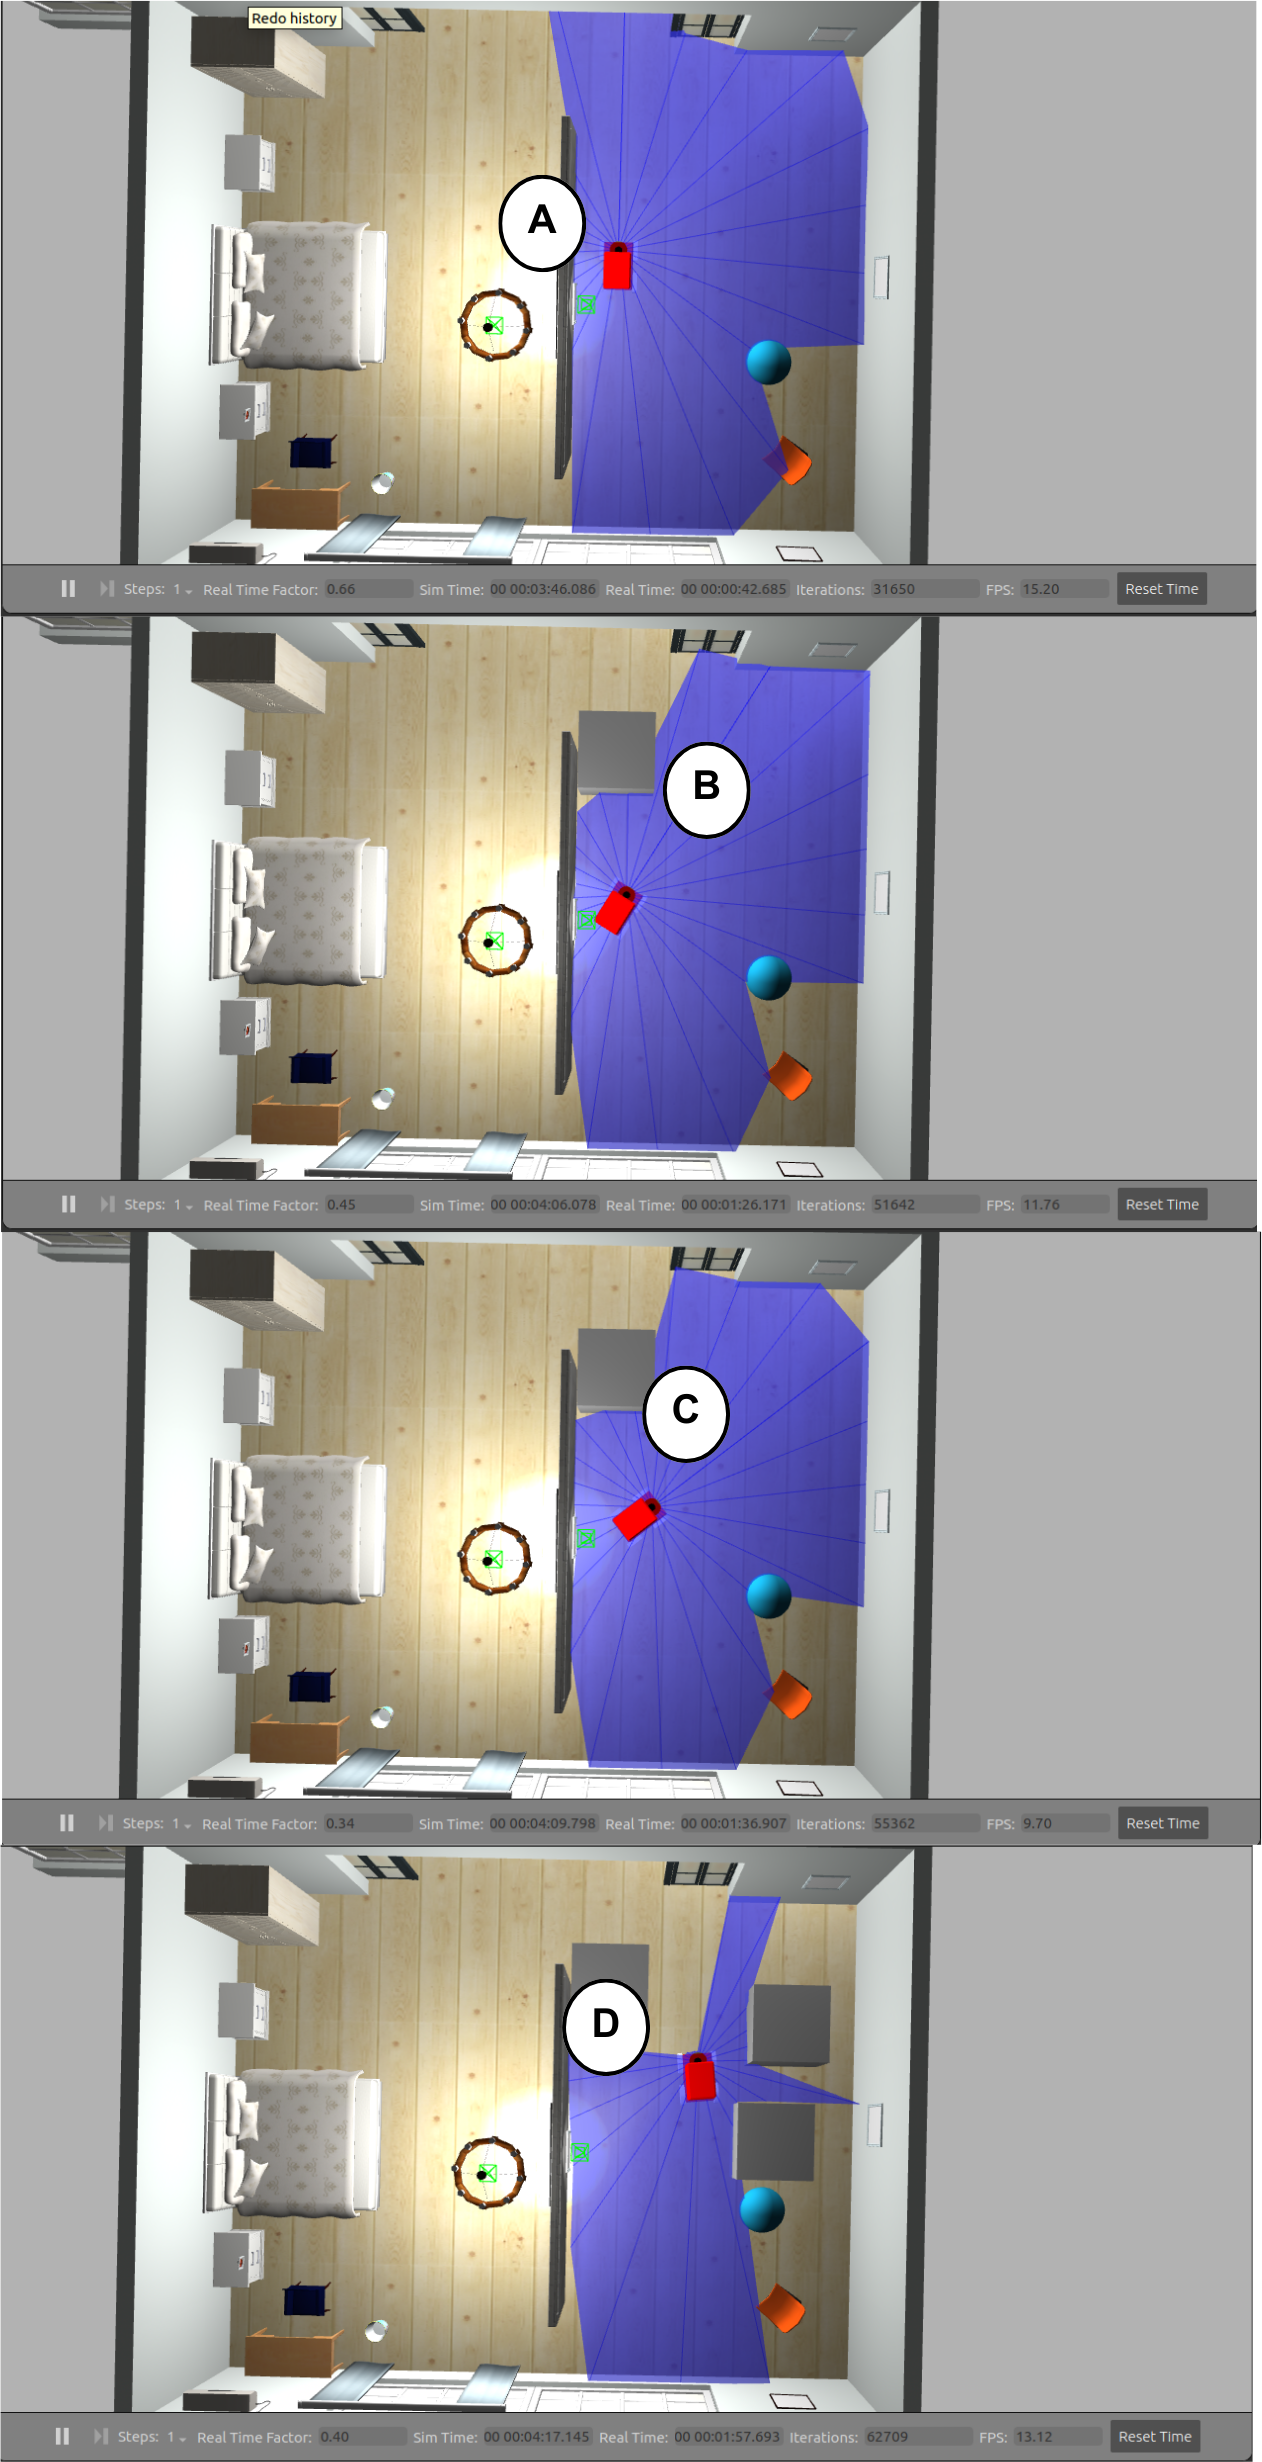
\includegraphics[scale=0.35]{ct01_1.png}
    \caption*{Fonte: Autora (2023).}
    \label{fig:ct01_1}
\end{figure}


\begin{figure}[H]
    \centering
    \caption{Captura da segunda repetição CT01}
    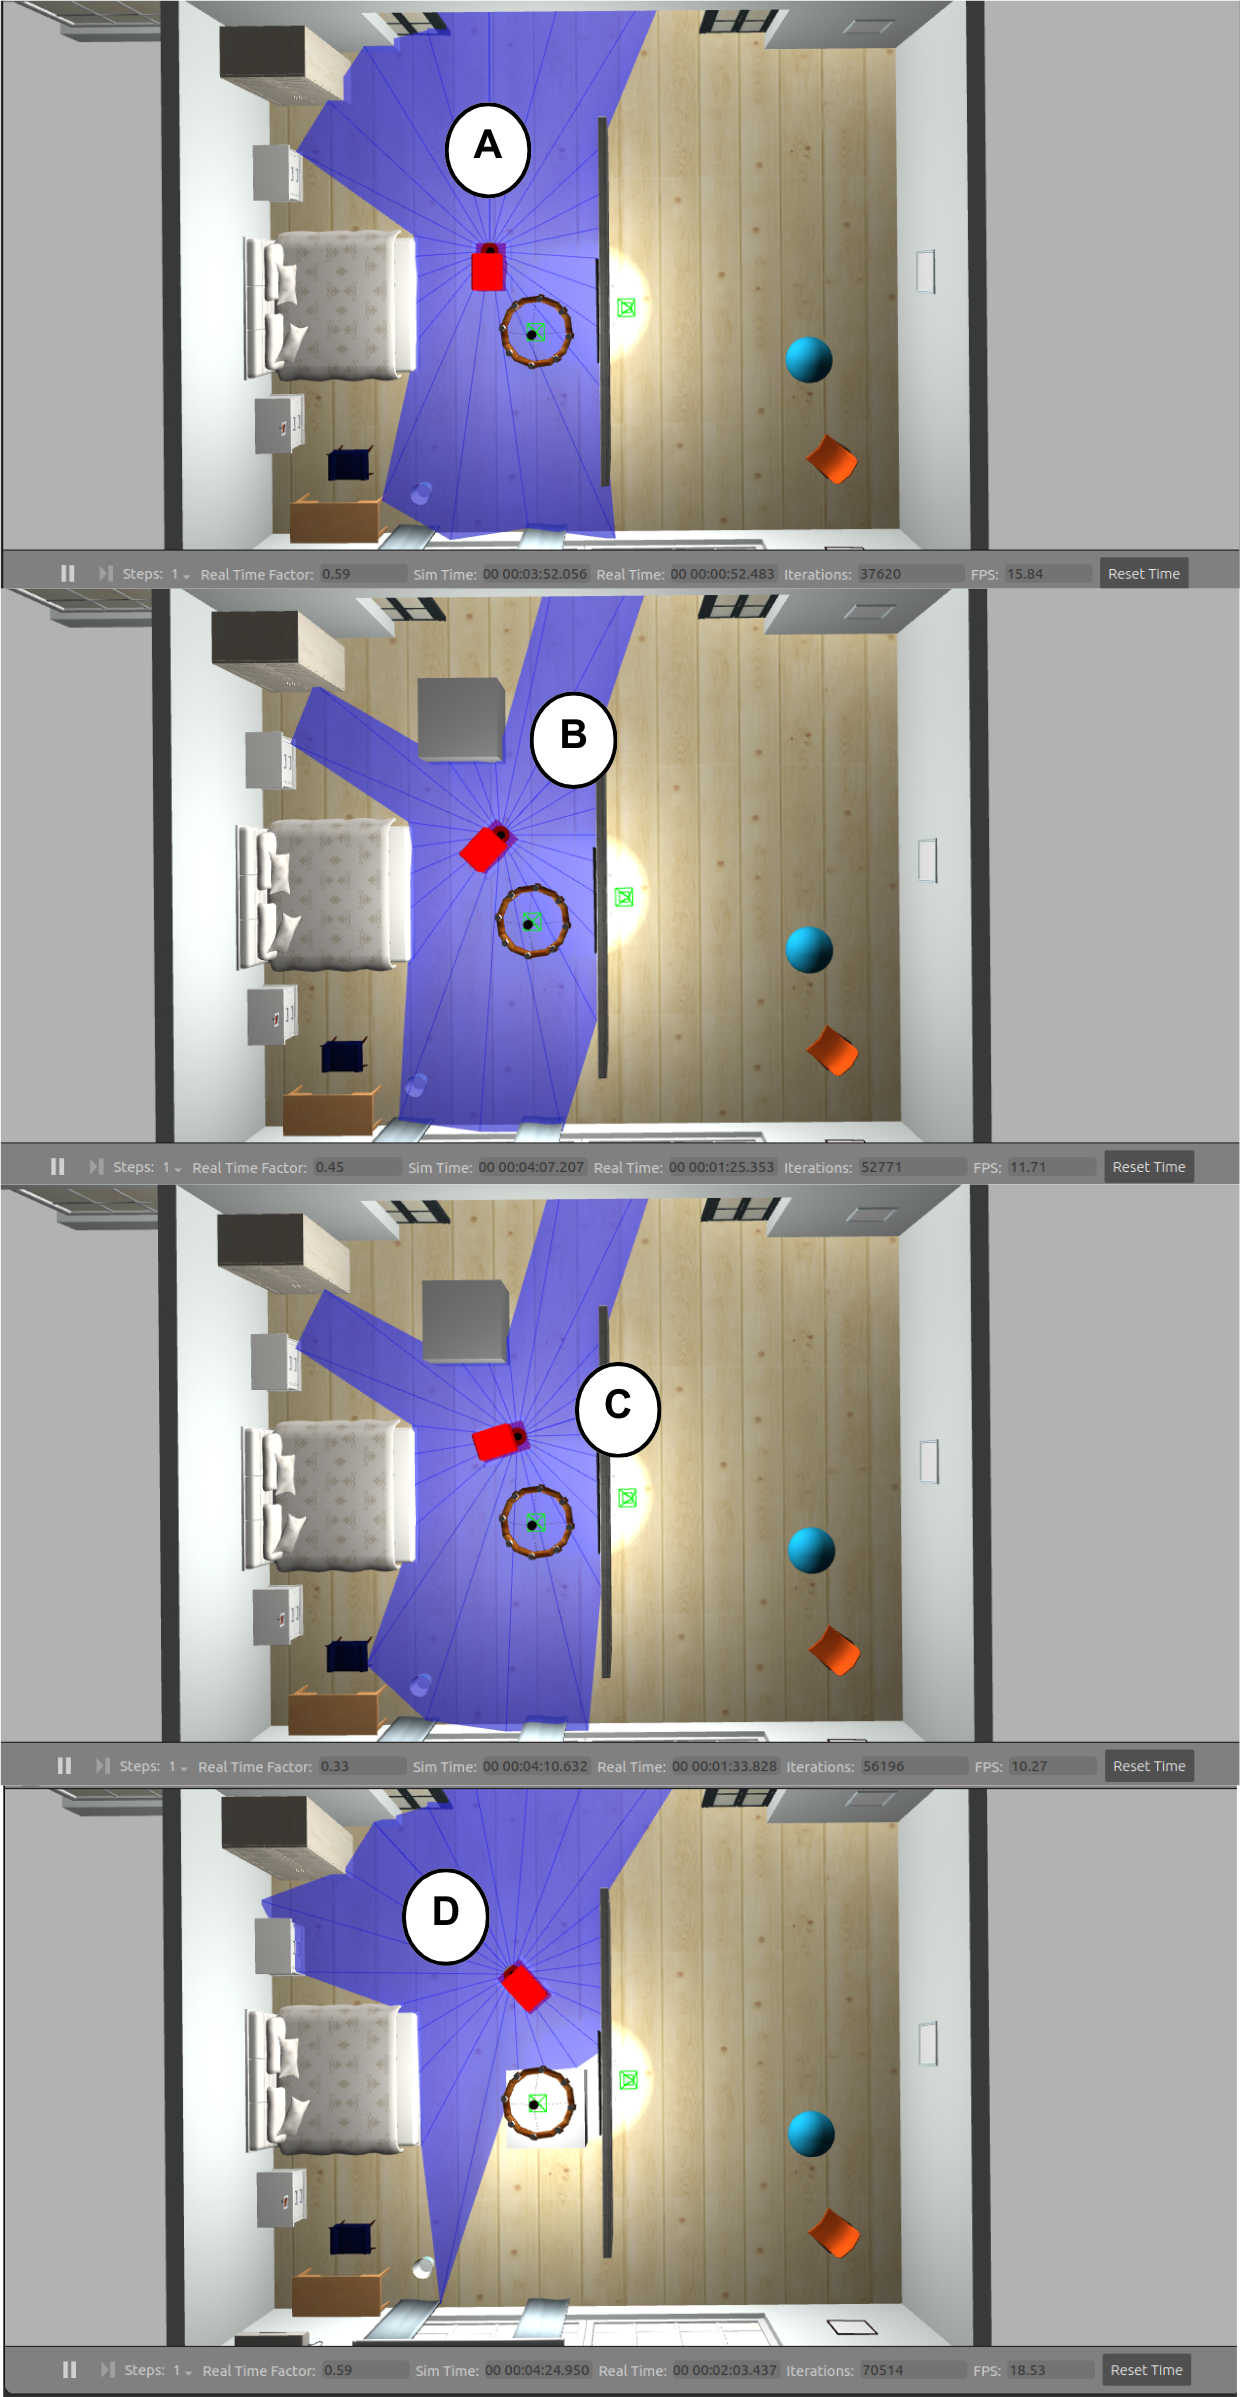
\includegraphics[scale=0.35]{ct01_2.png}
    \caption*{Fonte: Autora (2023).}
    \label{fig:ct01_2}
\end{figure}

\begin{figure}[H]
    \centering
    \caption{Captura da terceira repetição CT01}
    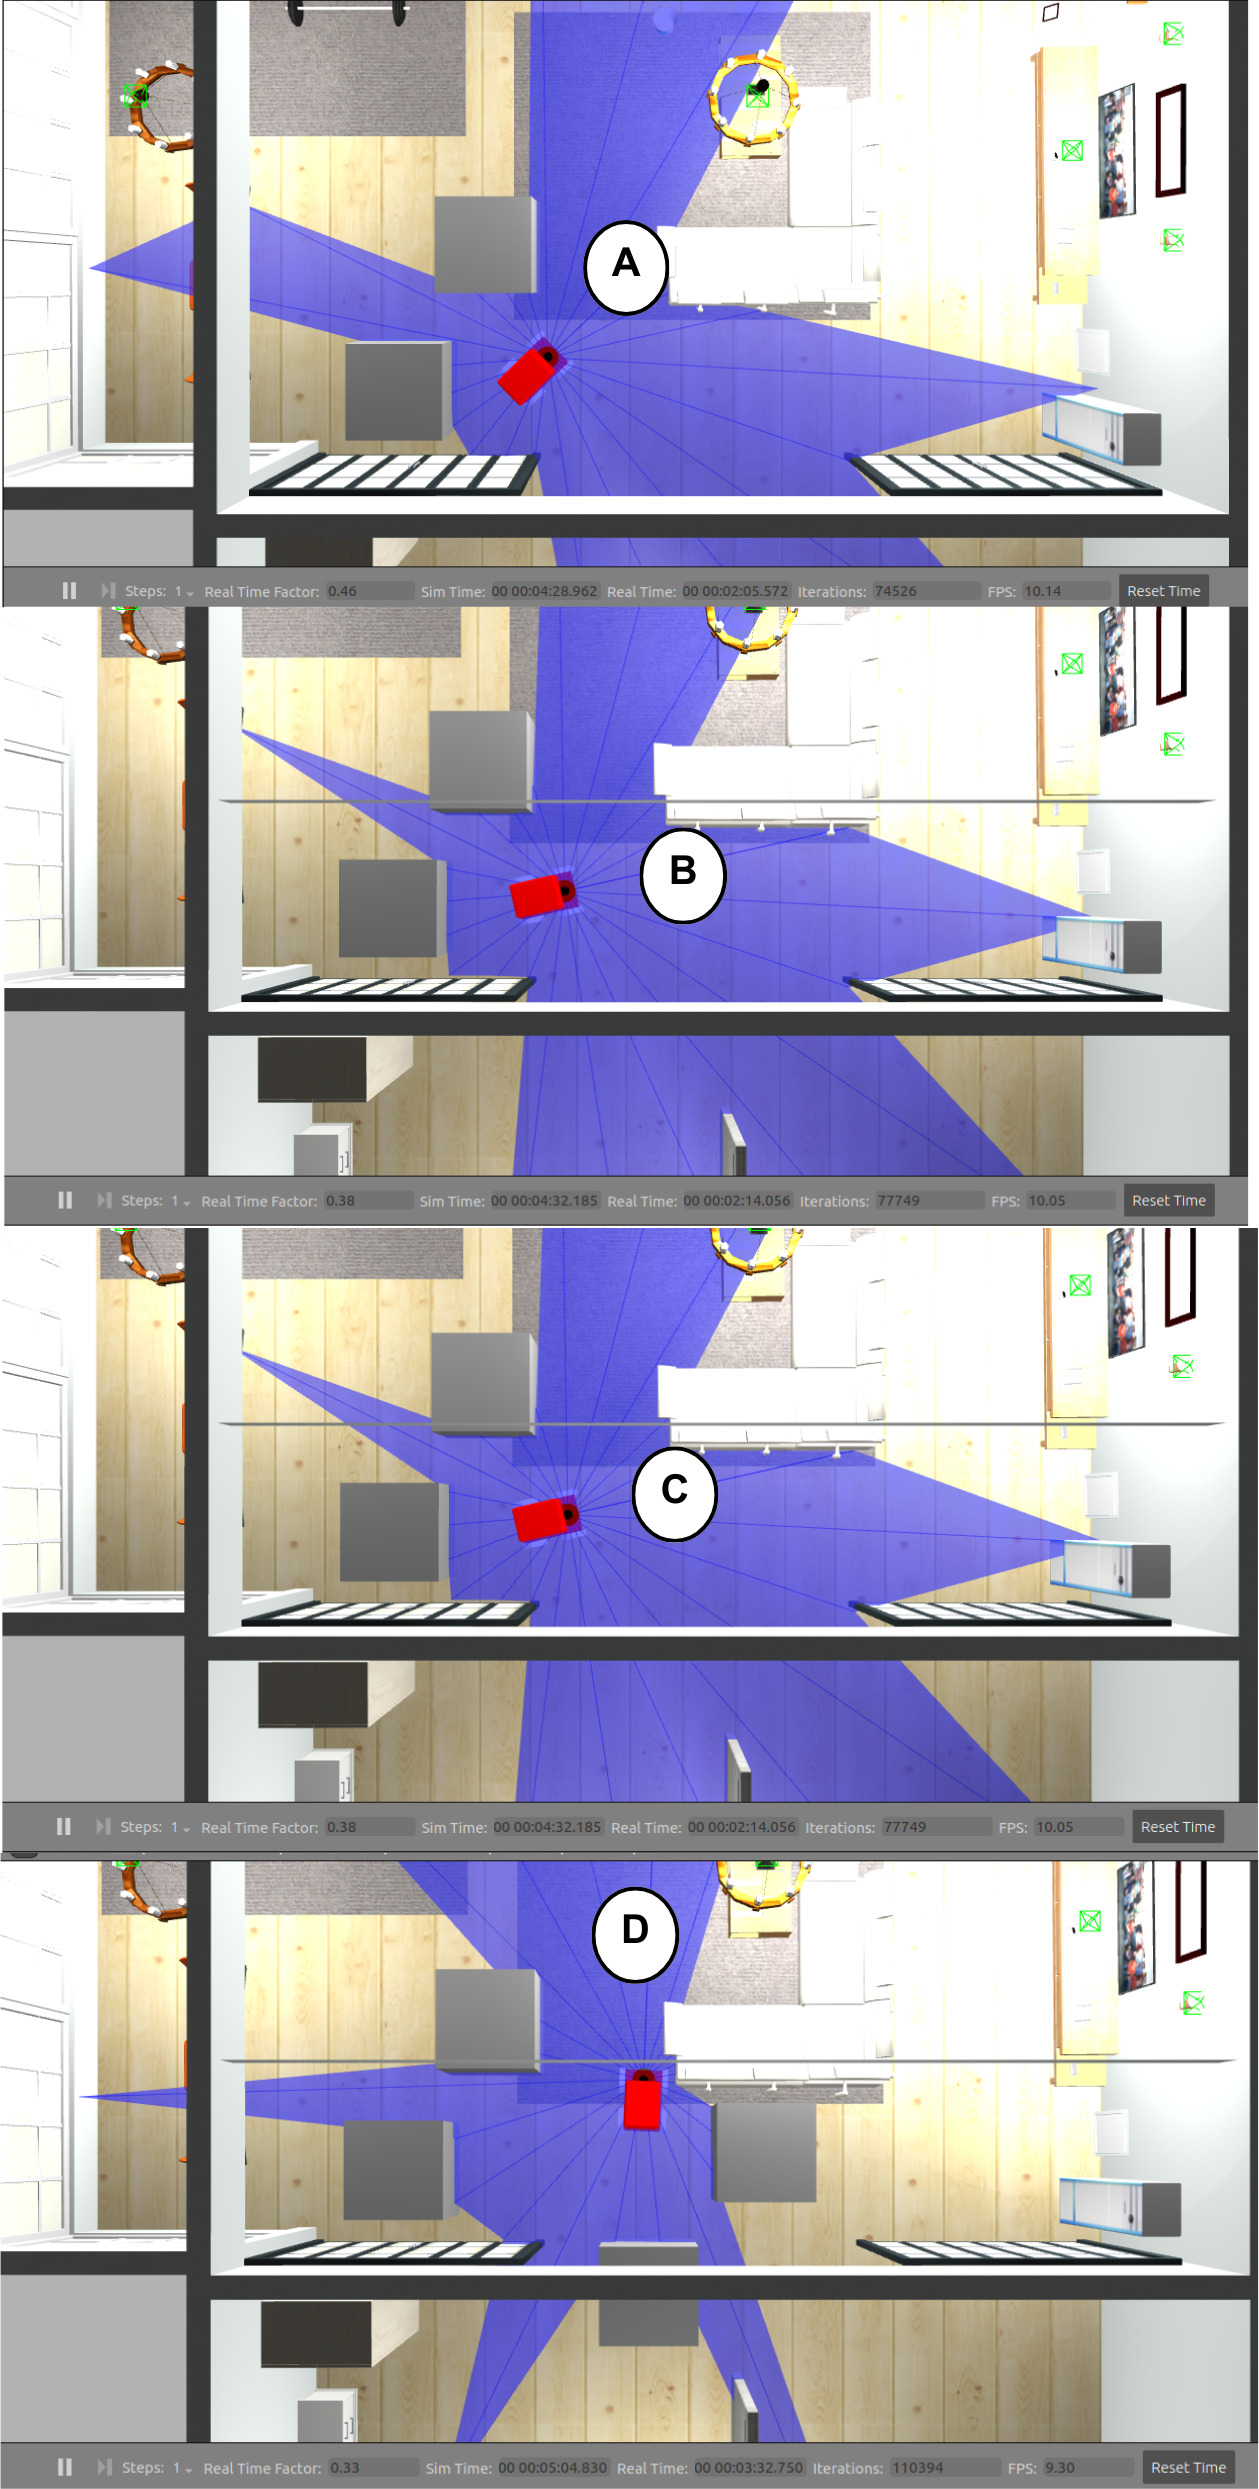
\includegraphics[scale=0.35]{ct01_3.png}
    \caption*{Fonte: Autora (2023).}
    \label{fig:ct01_3}
\end{figure}

\begin{figure}[H]
    \centering
    \caption{Captura da quarta repetição CT01}
    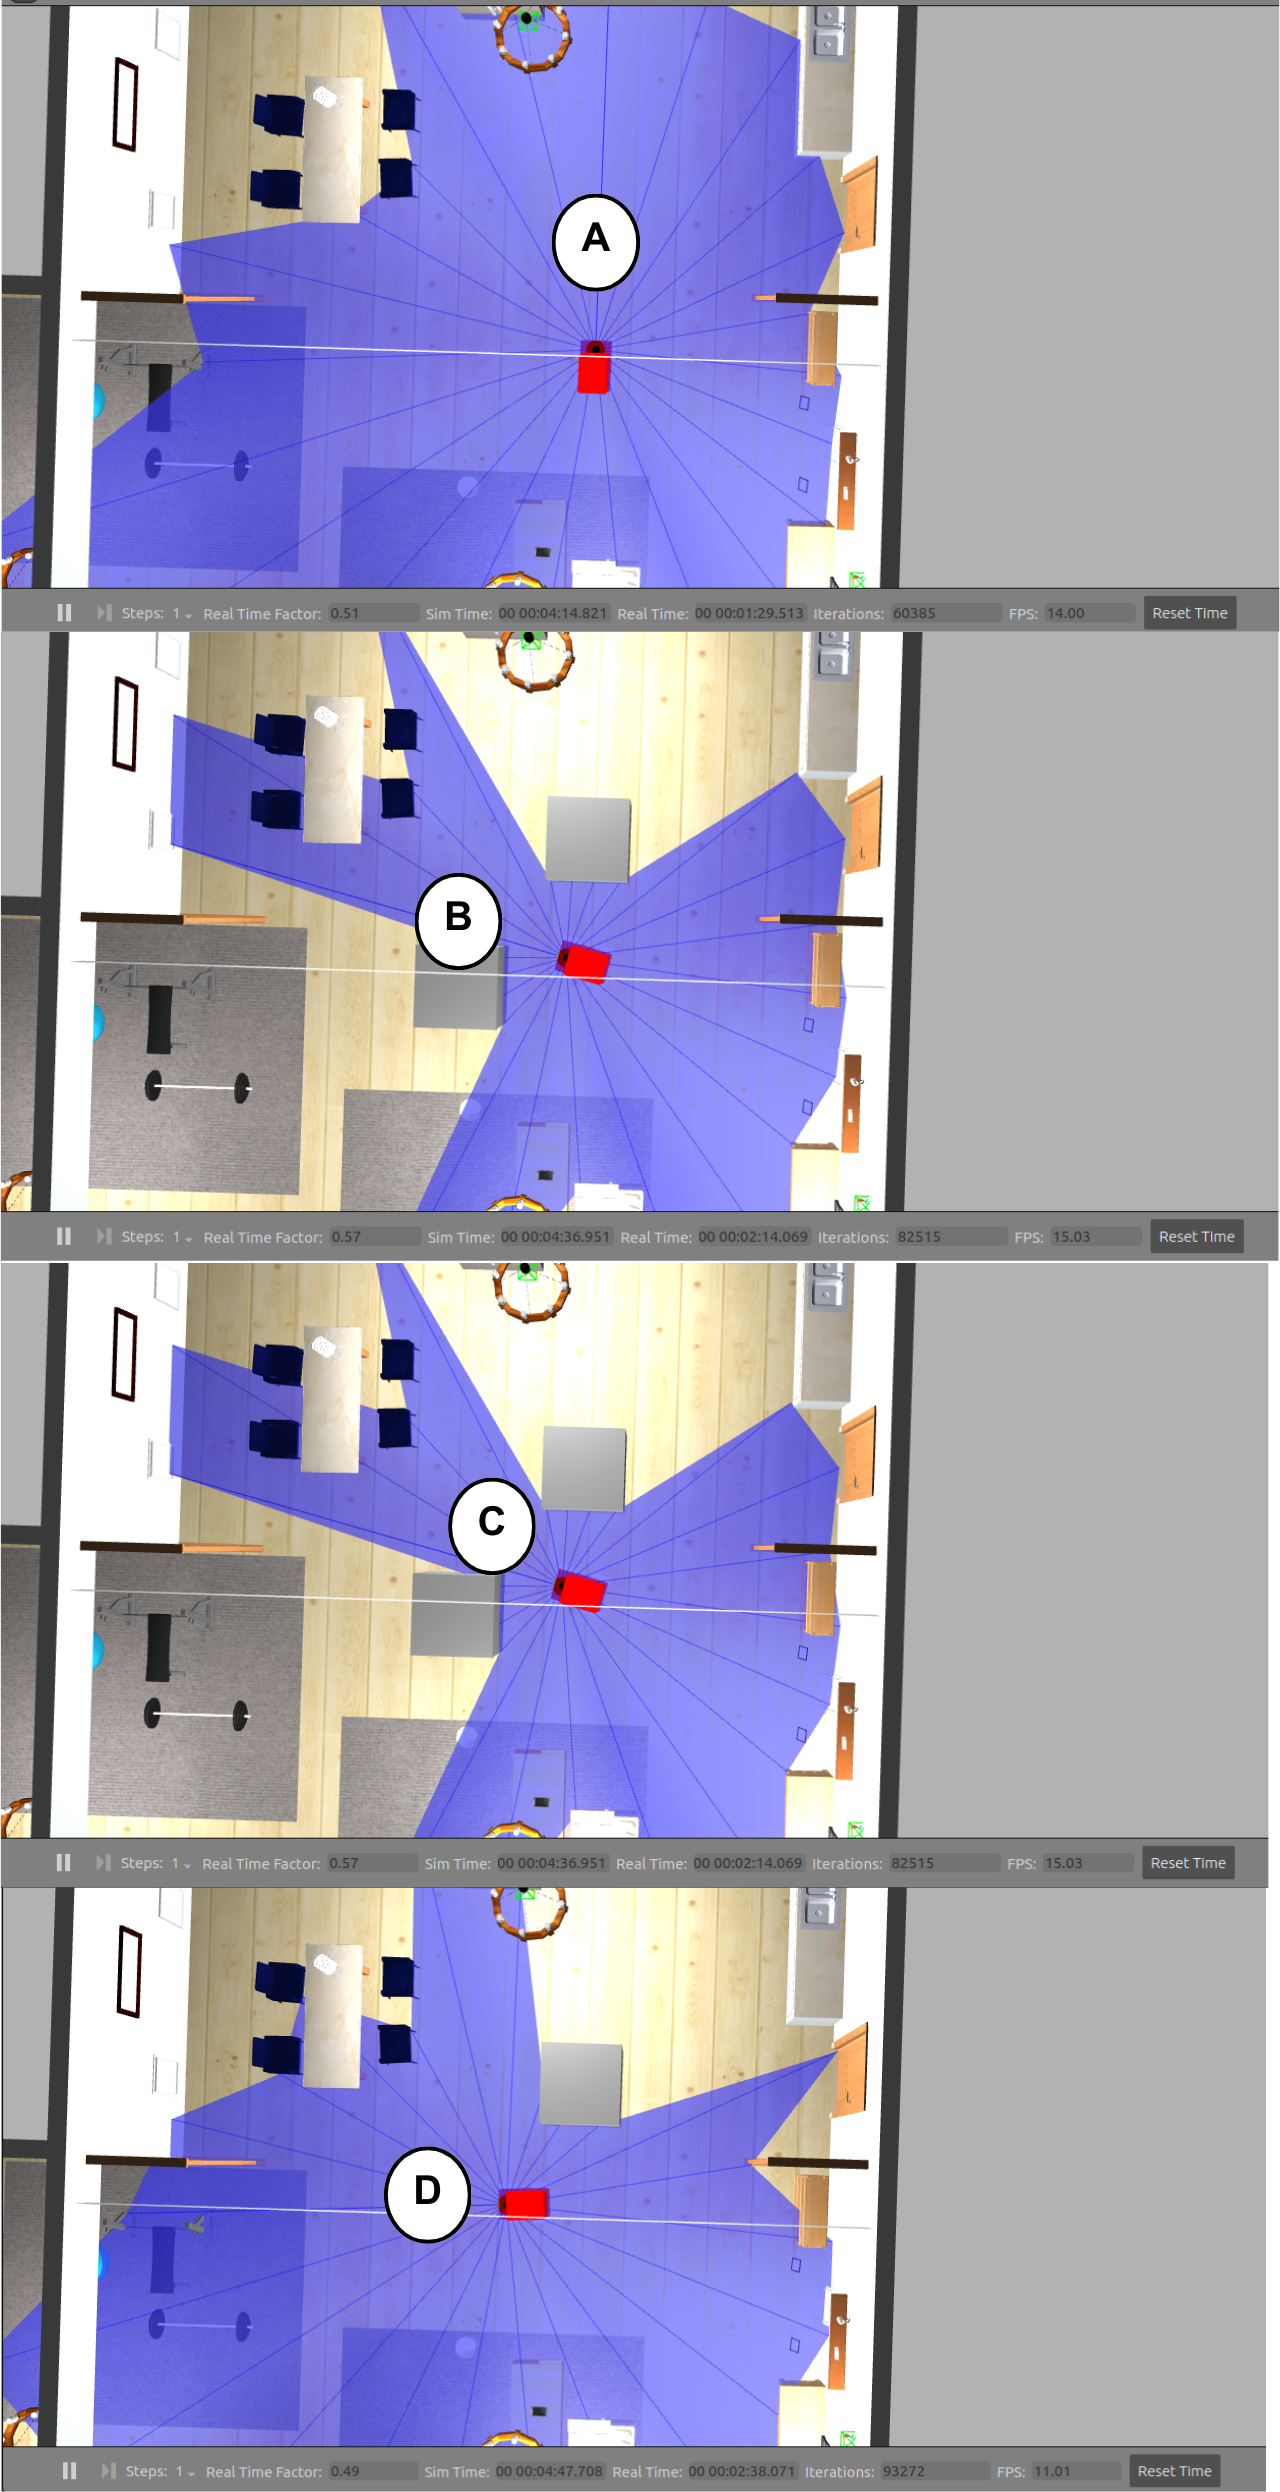
\includegraphics[scale=0.35]{ct01_4.png}
    \caption*{Fonte: Autora (2023).}
    \label{fig:ct01_4}
\end{figure}

\begin{figure}[H]
    \centering
    \caption{Captura da quinta repetição CT01}
    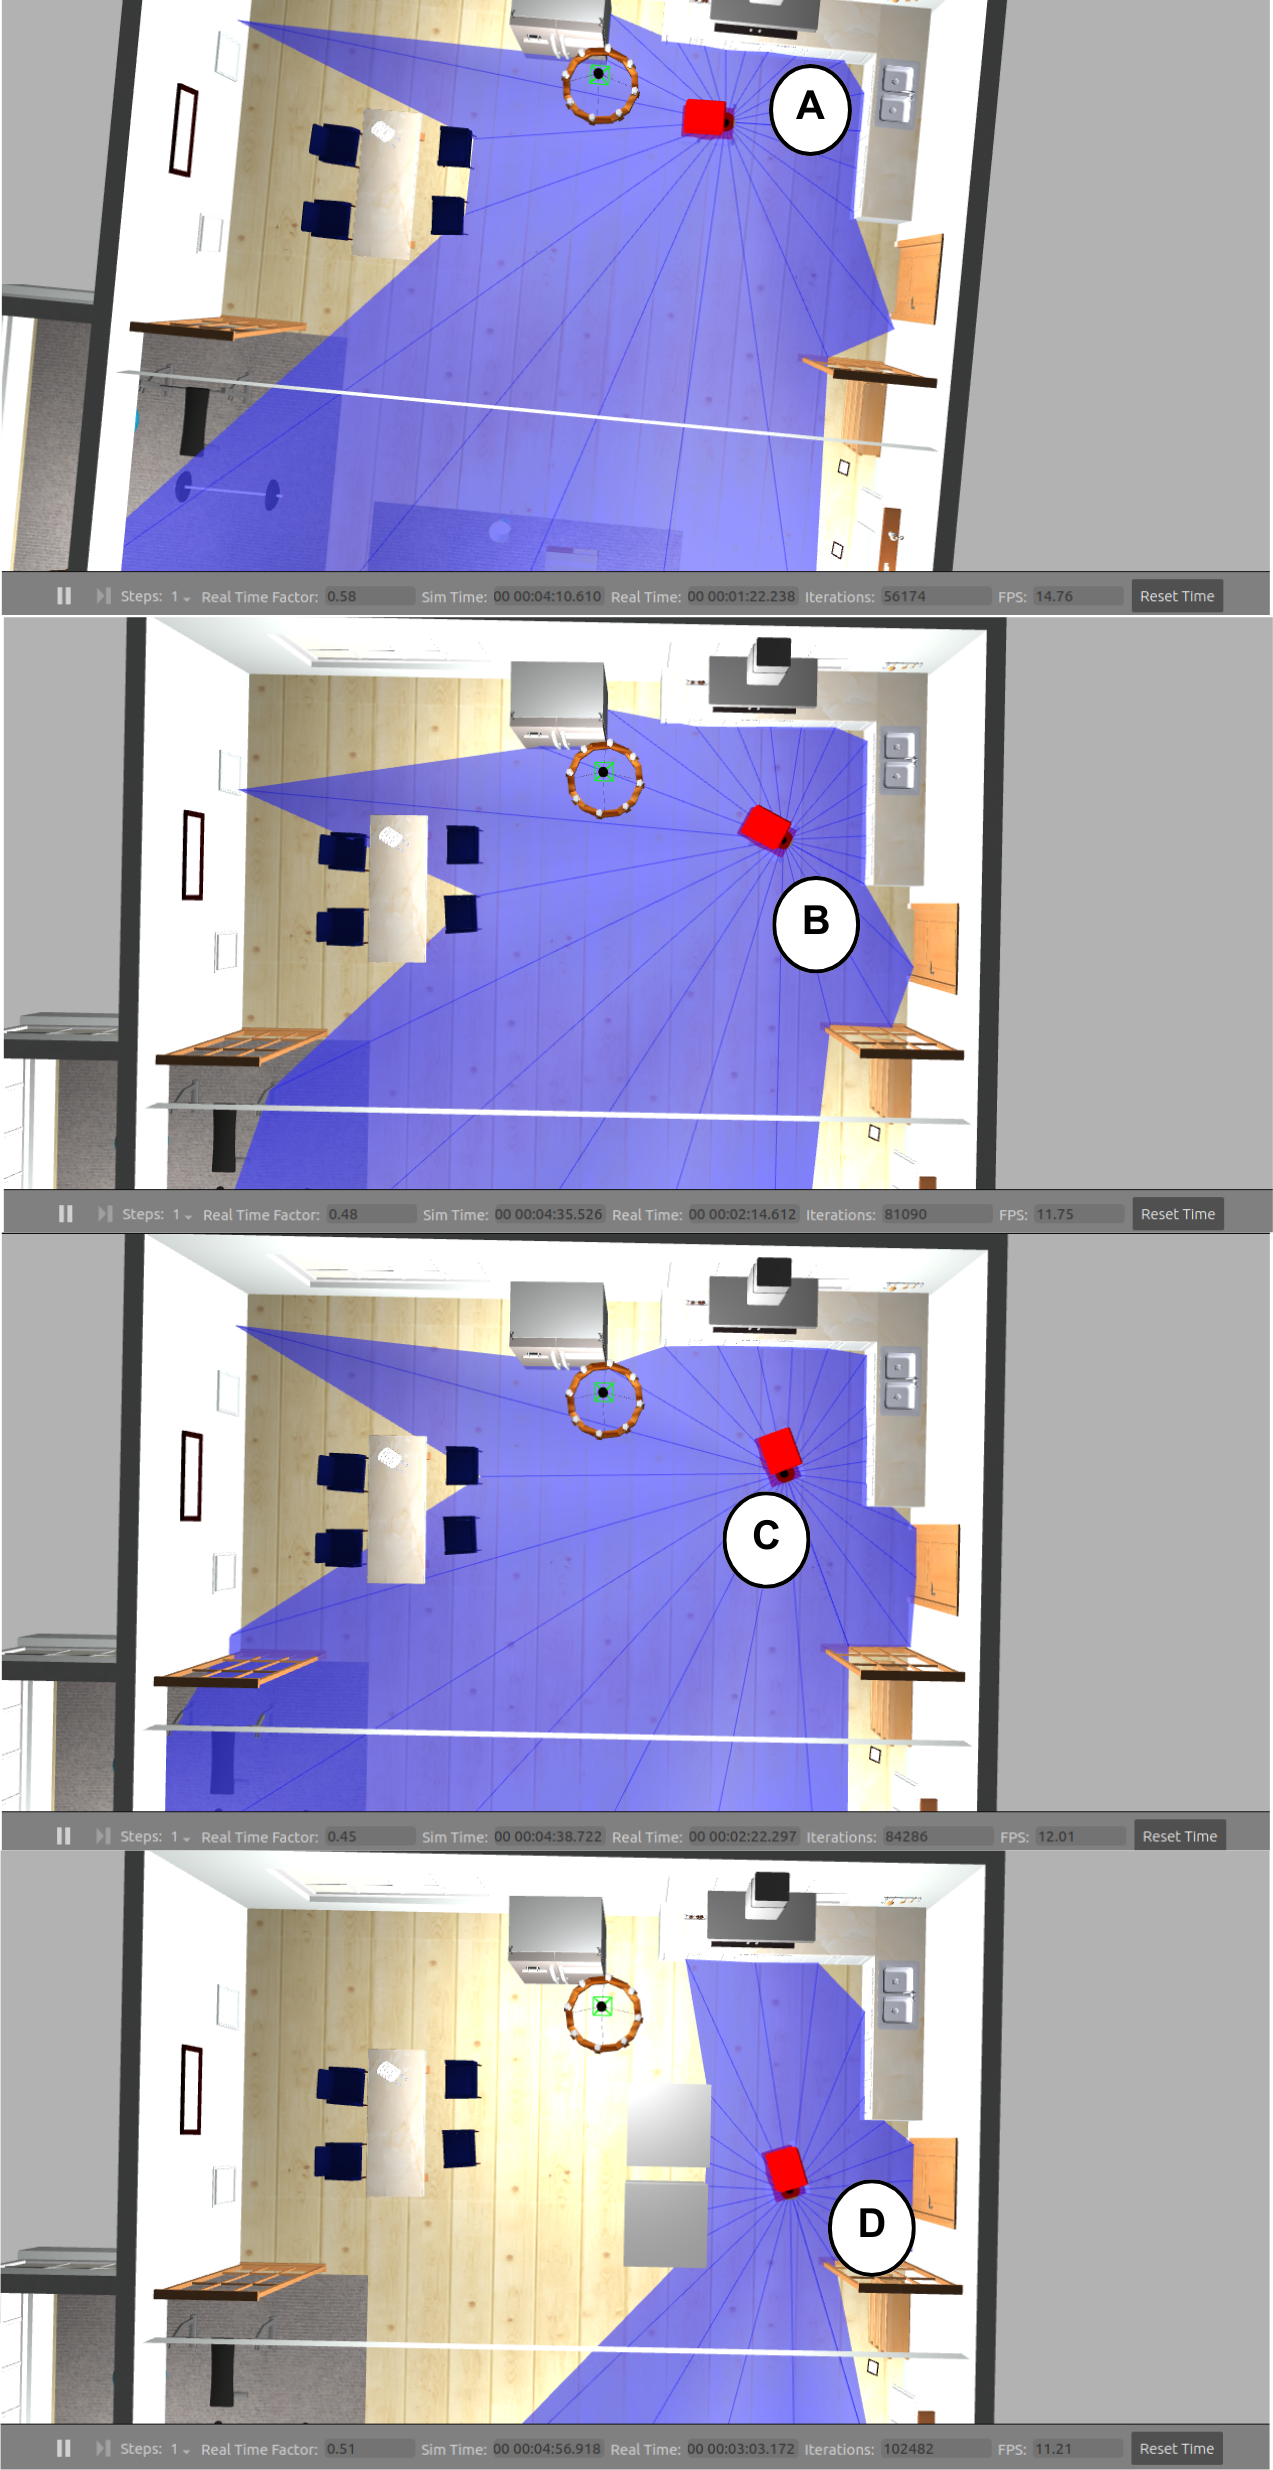
\includegraphics[scale=0.35]{ct01_5.png}
    \caption*{Fonte: Autora (2023).}
    \label{fig:ct01_5}
\end{figure}

\section{Caso de Teste CT02 Referente a RFS02}
O caso de teste CT02 teve o objetivo de identificar se o robô consegue se movimentar pelo ambiente sem colidir com nenhum obstáculo existente no seu caminho.  O caso de teste foi repetido cinco vezes com o robô em lugares distintos no ambiente. Entre os cinco testes, apenas um foi mal sucedido, visto que o robô se encontrava em um local estreito e não conseguiu continuar a trajetória. Todos os resultados podem ser visualizados na Tabela~\ref{tab:acertosct02}. Além disso, a seguir podem ser encontradas as capturas para cada repetição (Figura~\ref{fig:ct02_1}, Figura~\ref{fig:ct02_2}, Figura~\ref{fig:ct02_3}, Figura~\ref{fig:ct02_4}, Figura~\ref{fig:ct02_5}).


\begin{table}[H]
\centering
\caption{Resultados das repetições CT02}
\label{tab:acertosct02}
\resizebox{\textwidth}{!}{%
\begin{tabular}{l|c}
                              & \multicolumn{1}{l}{\textbf{Resultados CT02}} \\ \hline
\textbf{Teste 1}              & Bem-sucedido                                 \\
\textbf{Teste 2}              & Bem-sucedido                                 \\
\textbf{Teste 3}              & Bem-sucedido                                 \\
\textbf{Teste 4}              & Mal-sucedido                                 \\
\textbf{Teste 5}              & Bem-sucedido                                 \\
\textbf{Total de acertos (\%)} & \textbf{80}                                  \\ \hline
\end{tabular}%
}
\caption*{Fonte: Autora (2023).}
\end{table}

\begin{figure}[H]
    \centering
    \caption{Captura da primeira repetição CT02}
    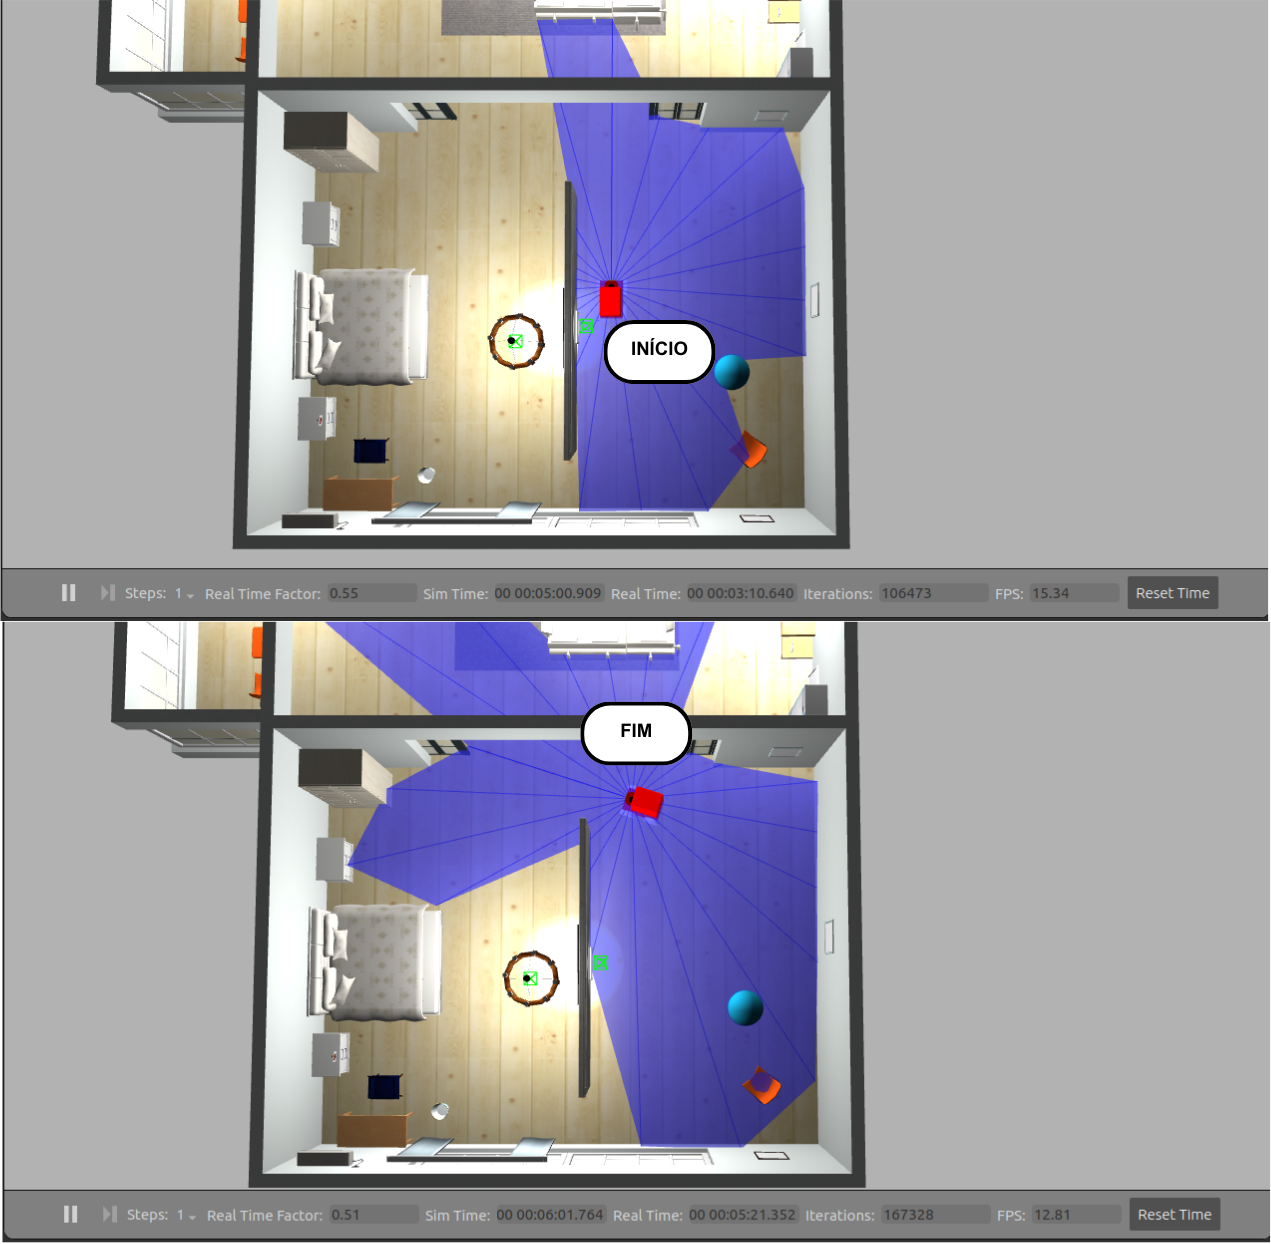
\includegraphics[scale=0.5]{ct02_1.png}
    \caption*{Fonte: Autora (2023).}
    \label{fig:ct02_1}
\end{figure}


\begin{figure}[H]
    \centering
    \caption{Captura da segunda repetição CT02}
    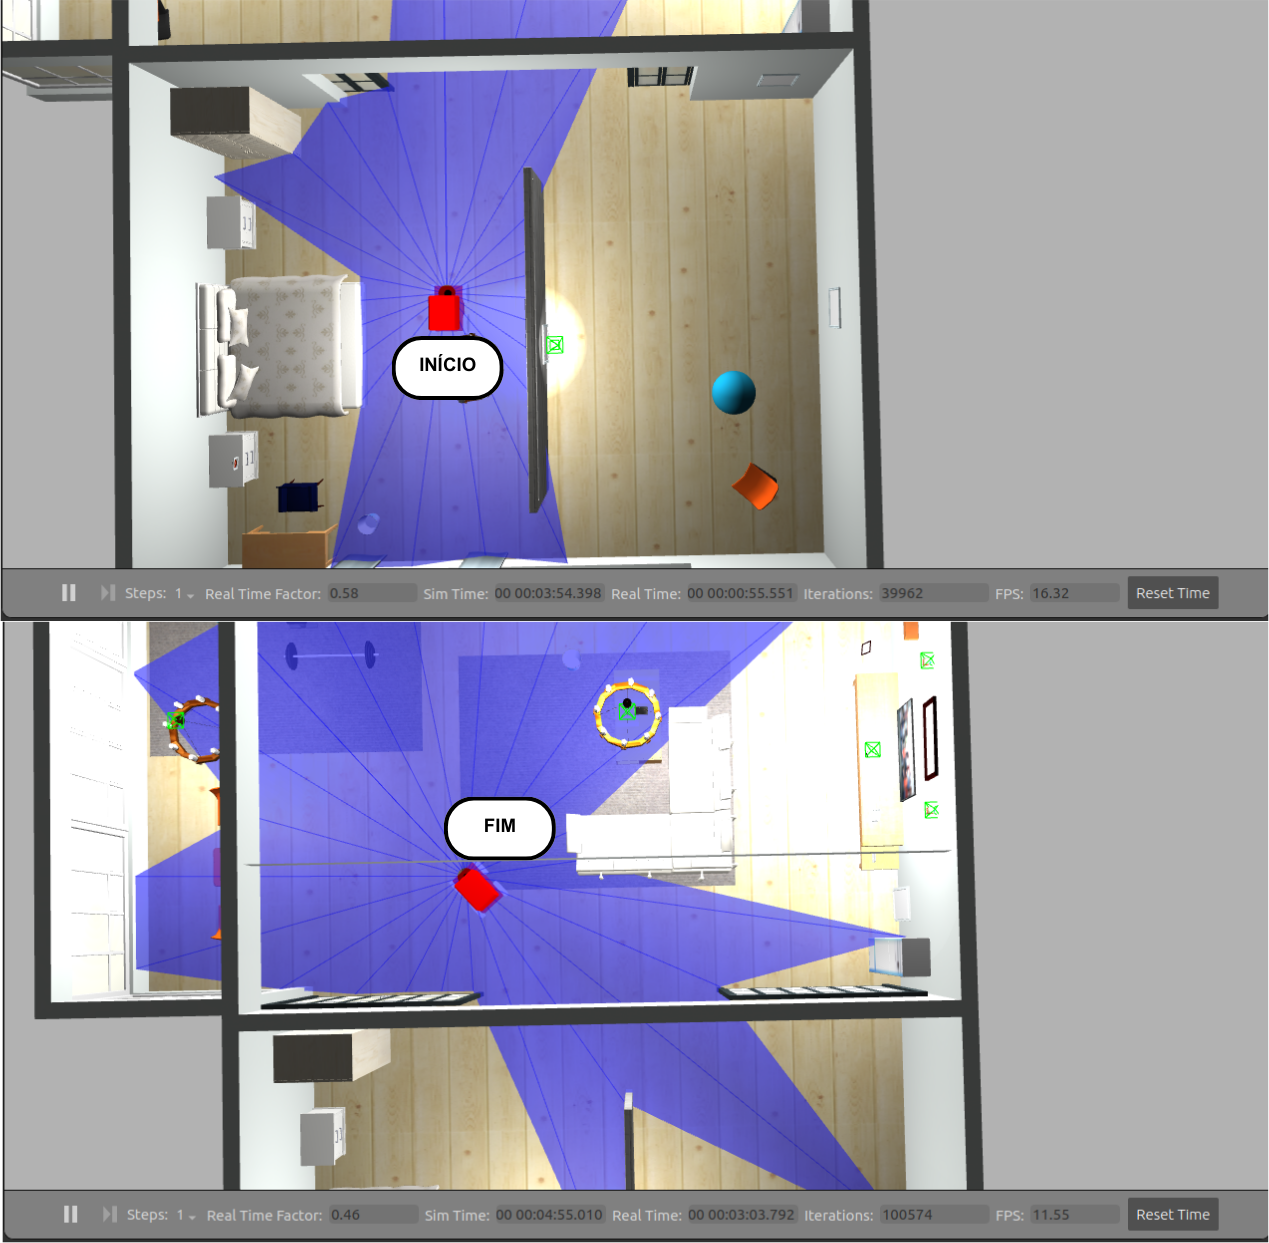
\includegraphics[scale=0.5]{ct02_2.png}
    \caption*{Fonte: Autora (2023).}
    \label{fig:ct02_2}
\end{figure}

\begin{figure}[H]
    \centering
    \caption{Captura da terceira repetição CT02}
    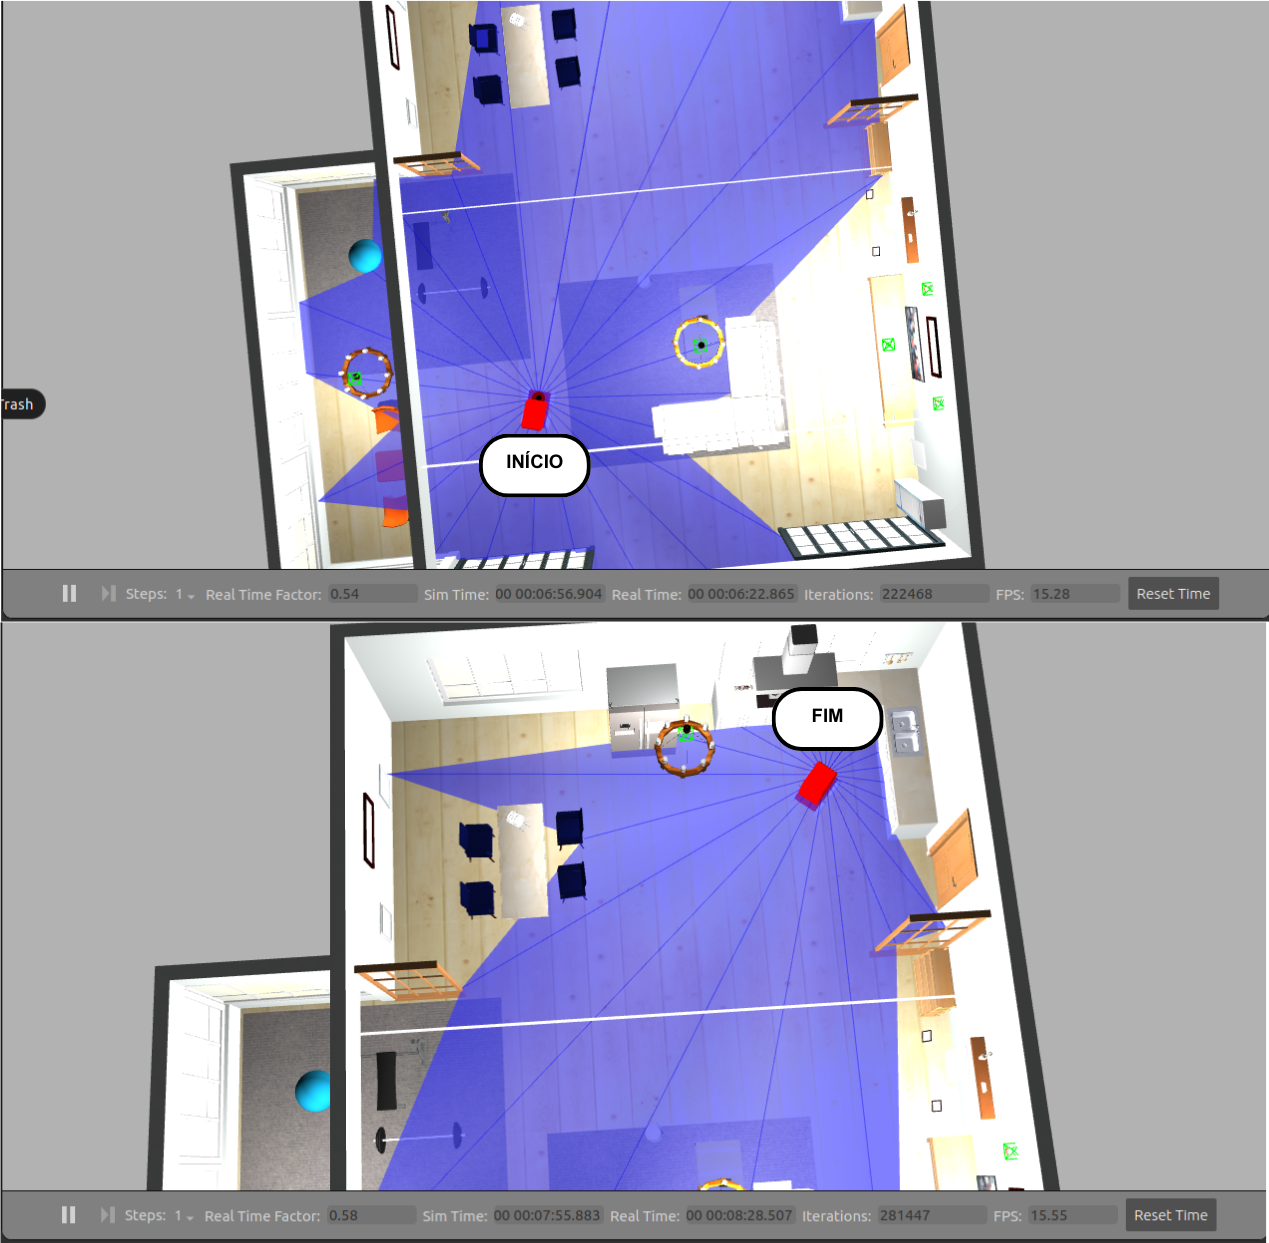
\includegraphics[scale=0.5]{ct02_3.png}
    \caption*{Fonte: Autora (2023).}
    \label{fig:ct02_3}
\end{figure}

\begin{figure}[H]
    \centering
    \caption{Captura da quarta repetição CT02}
    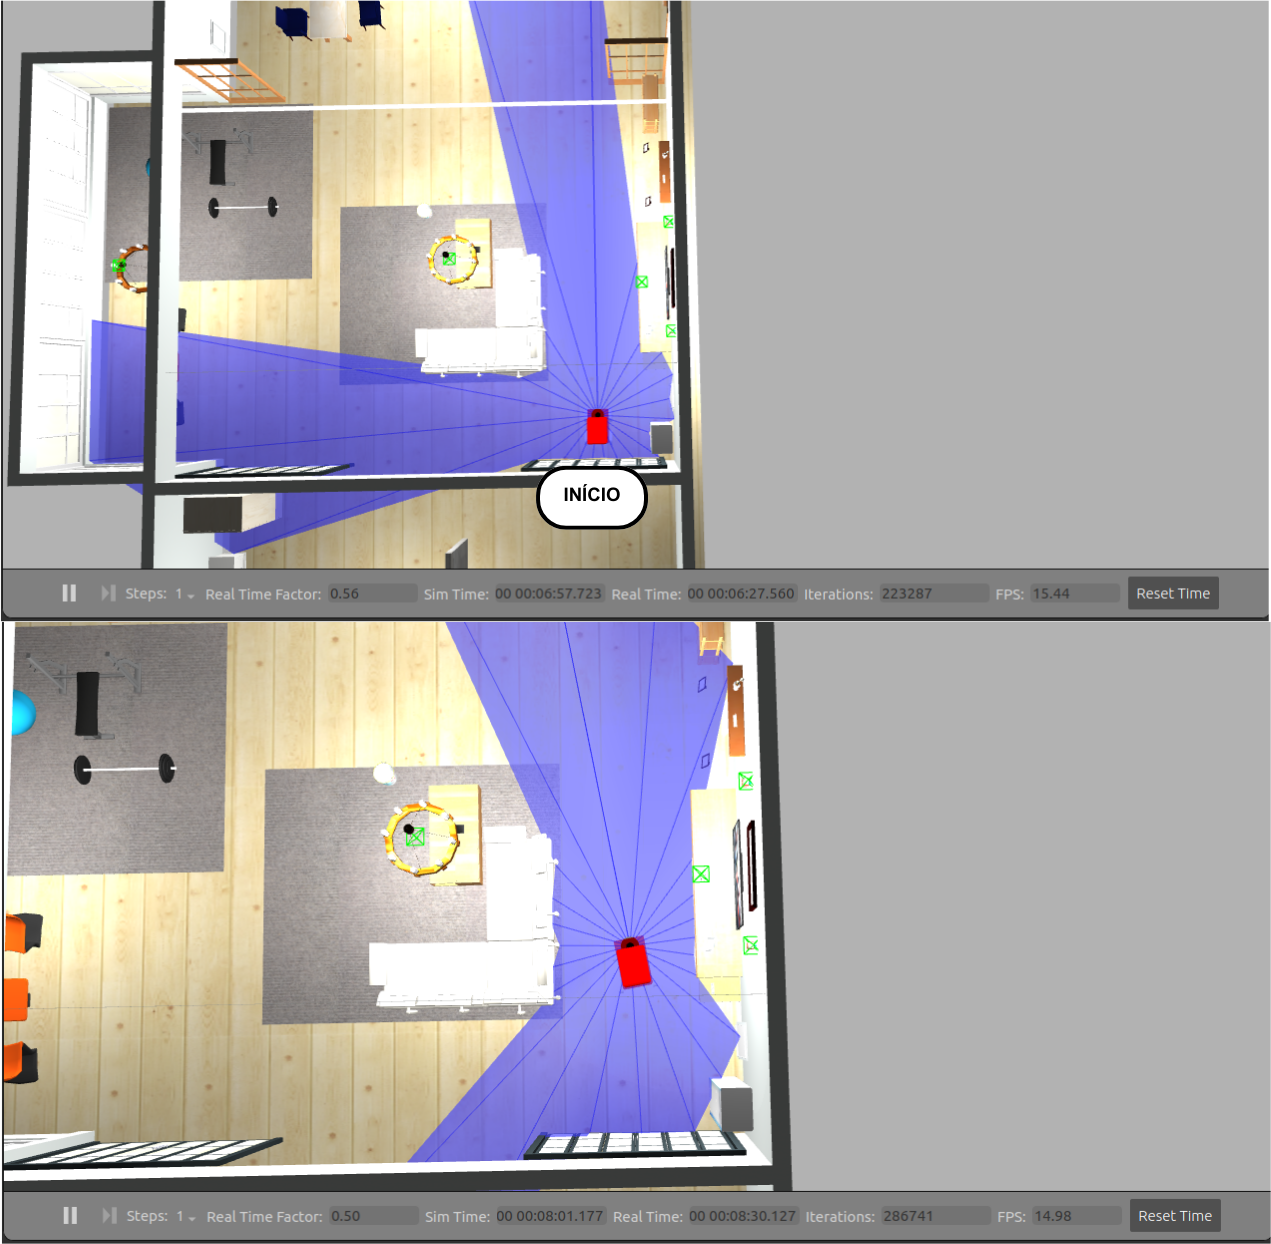
\includegraphics[scale=0.5]{ct02_4.png}
    \caption*{Fonte: Autora (2023).}
    \label{fig:ct02_4}
\end{figure}

\begin{figure}[H]
    \centering
    \caption{Captura da quinta repetição CT02}
    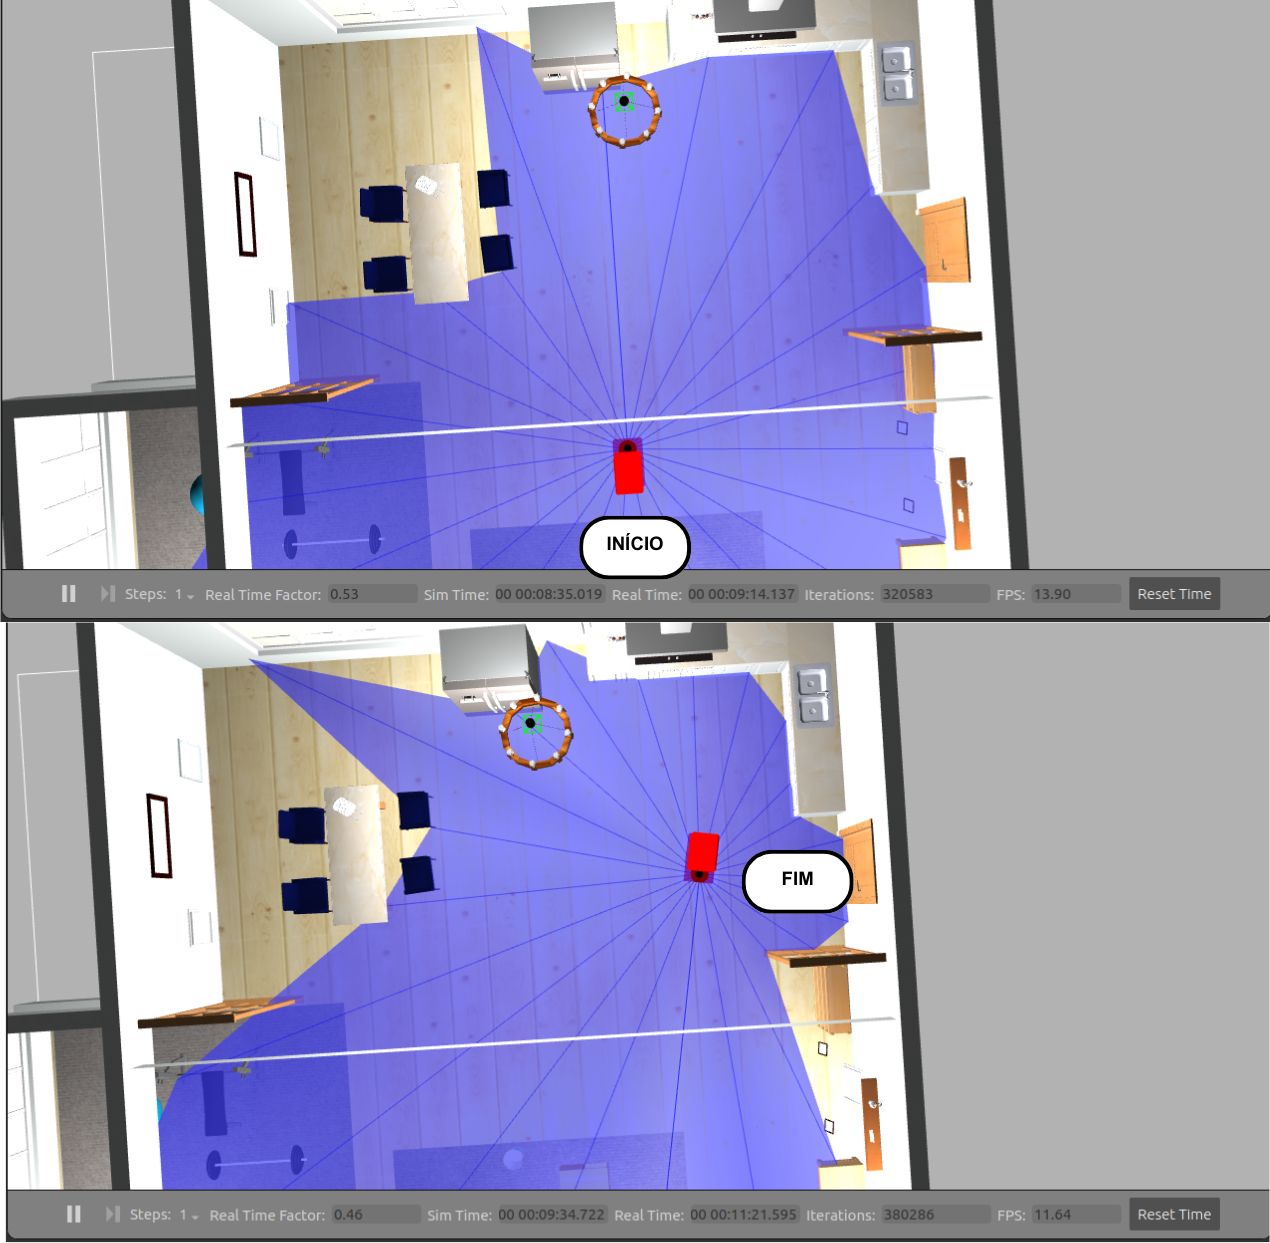
\includegraphics[scale=0.5]{ct02_5.png}
    \caption*{Fonte: Autora (2023).}
    \label{fig:ct02_5}
\end{figure}

\section{Caso de Teste CT03 Referente a RNFS01}
O caso de teste CT03 visou validar a locomoção do robô em superfície de piso liso e com tapete. O caso de teste foi repetido cinco vezes com o robô em lugares distintos no ambiente. Todos os cinco testes foram bem sucedidos. Todos os resultados podem ser visualizados na Tabela~\ref{tab:acertosct03}. Além disso, a seguir podem ser encontradas as capturas para cada repetição (Figura~\ref{fig:ct03_1}, Figura~\ref{fig:ct03_2}, Figura~\ref{fig:ct03_3}, Figura~\ref{fig:ct03_4}, Figura~\ref{fig:ct03_5}).


\begin{table}[H]
\centering
\caption{Resultados das Repetições CT03}
\label{tab:acertosct03}
\resizebox{\textwidth}{!}{%
\begin{tabular}{l|c}
                              & \multicolumn{1}{l}{\textbf{Resultados CT03}} \\ \hline
\textbf{Teste 1}              & Bem-sucedido                                 \\
\textbf{Teste 2}              & Bem-sucedido                                 \\
\textbf{Teste 3}              & Bem-sucedido                                 \\
\textbf{Teste 4}              & Bem-sucedido                                 \\
\textbf{Teste 5}              & Bem-sucedido                                 \\
\textbf{Total de acertos (\%)} & \textbf{100}                                  \\ \hline
\end{tabular}%
}
\caption*{Fonte: Autora (2023).}
\end{table}

\begin{figure}[H]
    \centering
    \caption{Captura da primeira repetição CT03}
    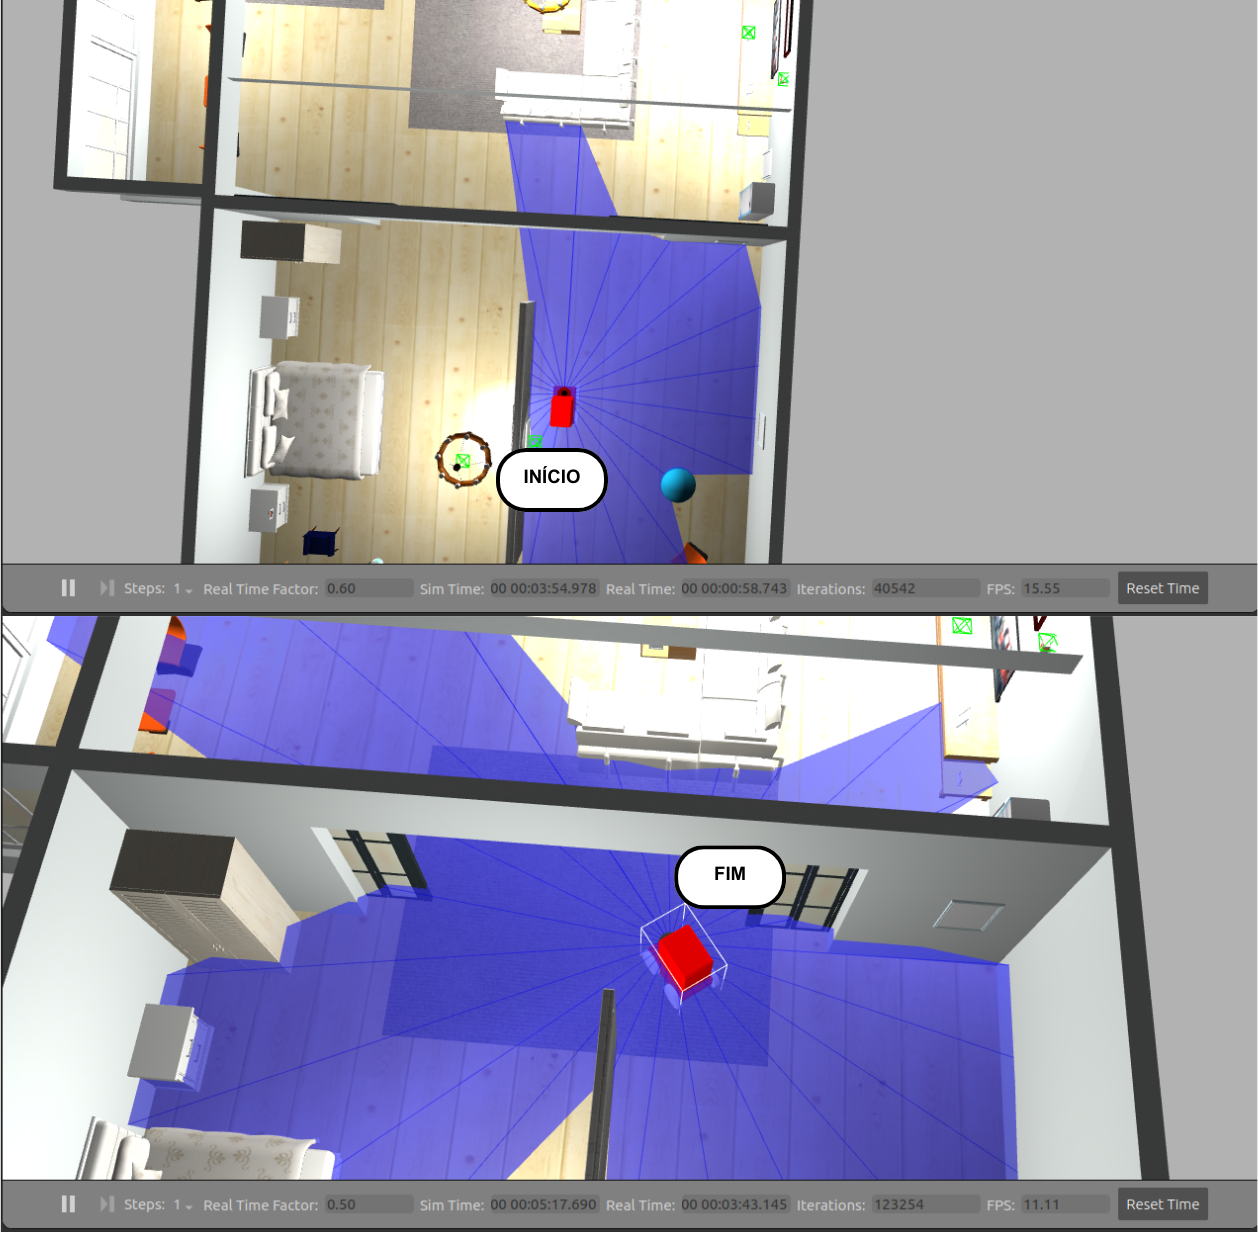
\includegraphics[scale=0.5]{ct03_1.png}
    \caption*{Fonte: Autora (2023).}
    \label{fig:ct03_1}
\end{figure}


\begin{figure}[H]
    \centering
    \caption{Captura da segunda repetição CT03}
    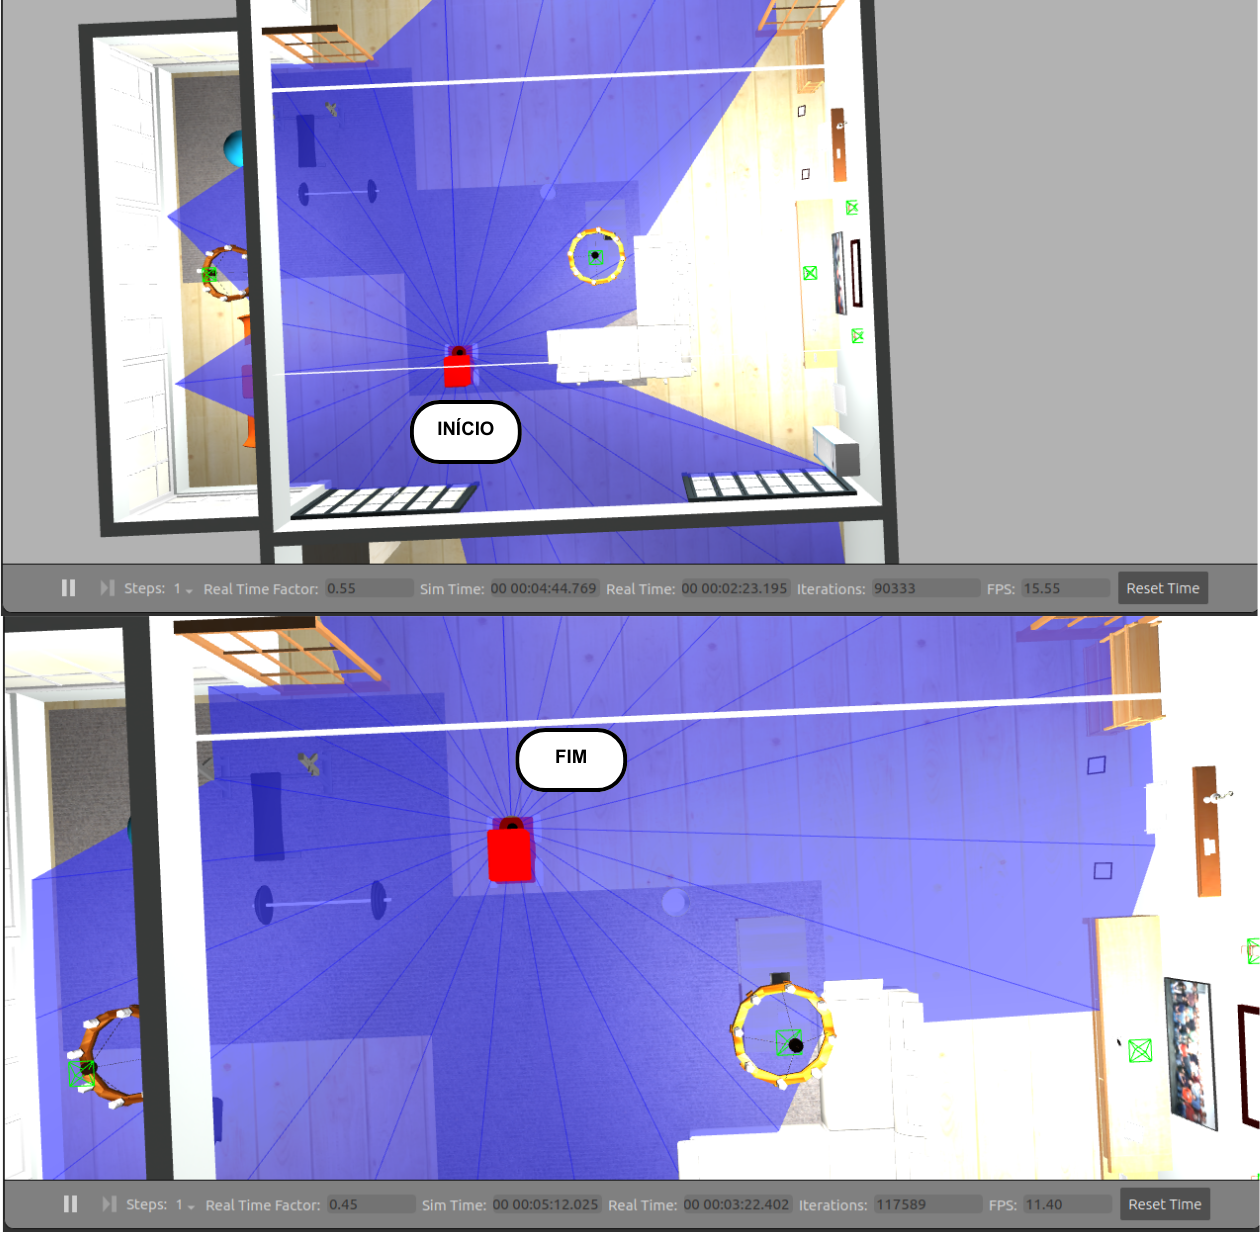
\includegraphics[scale=0.5]{ct03_2.png}
    \caption*{Fonte: Autora (2023).}
    \label{fig:ct03_2}
\end{figure}

\begin{figure}[H]
    \centering
    \caption{Captura da terceira repetição CT03}
    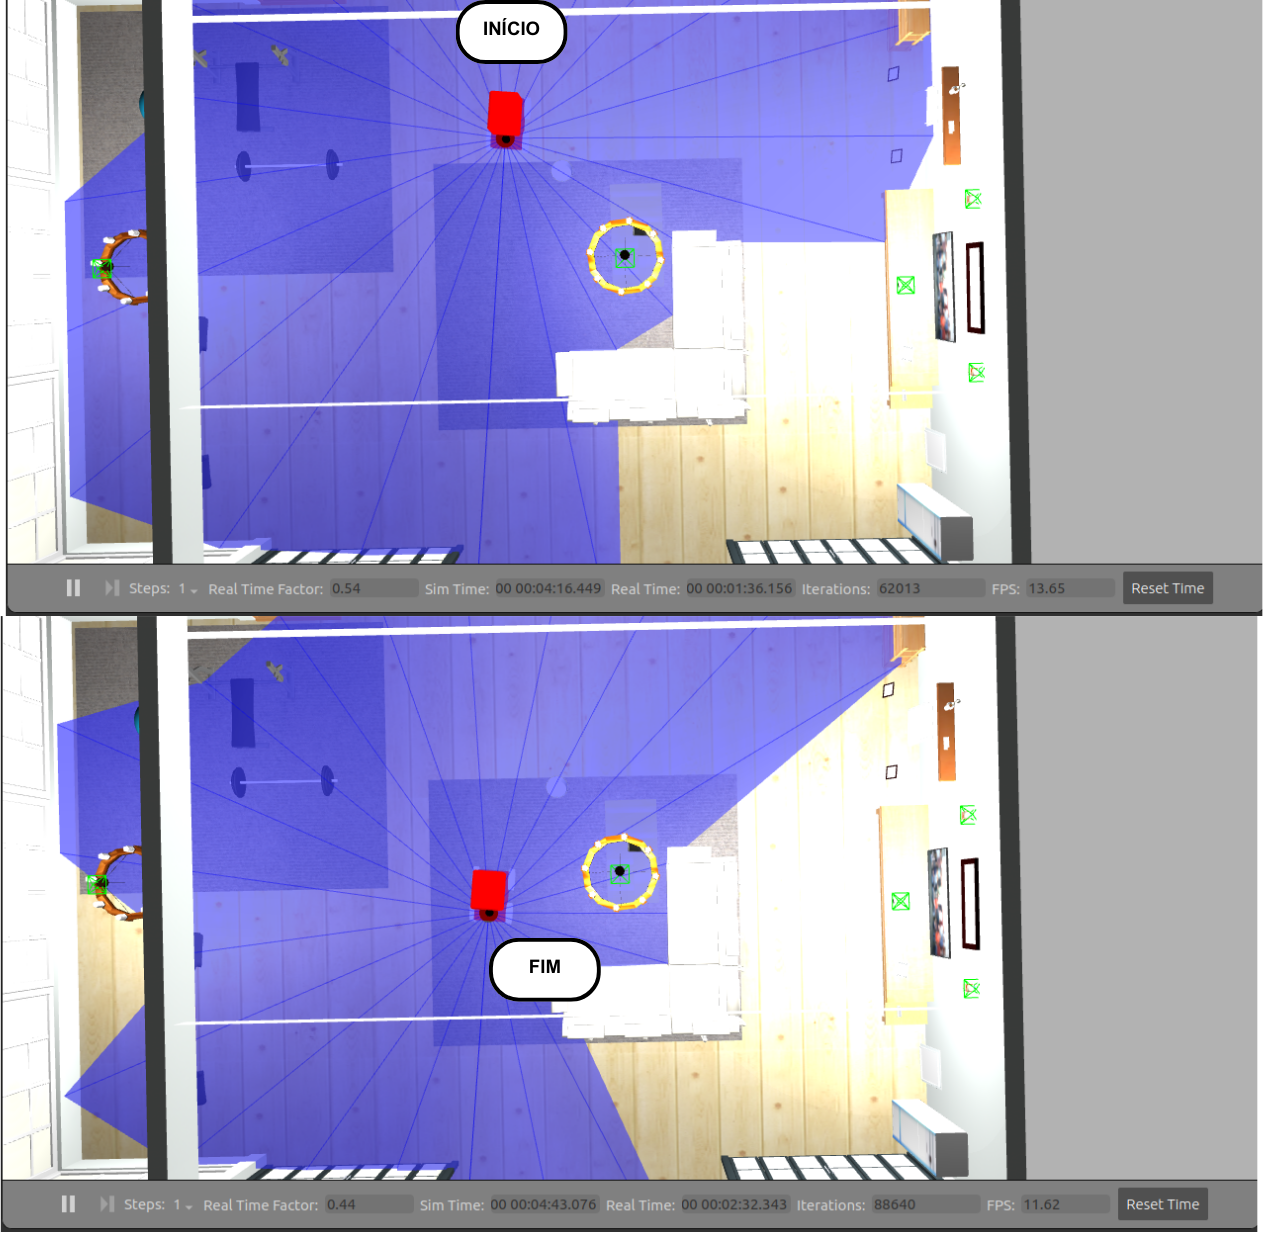
\includegraphics[scale=0.5]{ct03_3.png}
    \caption*{Fonte: Autora (2023).}
    \label{fig:ct03_3}
\end{figure}

\begin{figure}[H]
    \centering
    \caption{Captura da quarta repetição CT03}
    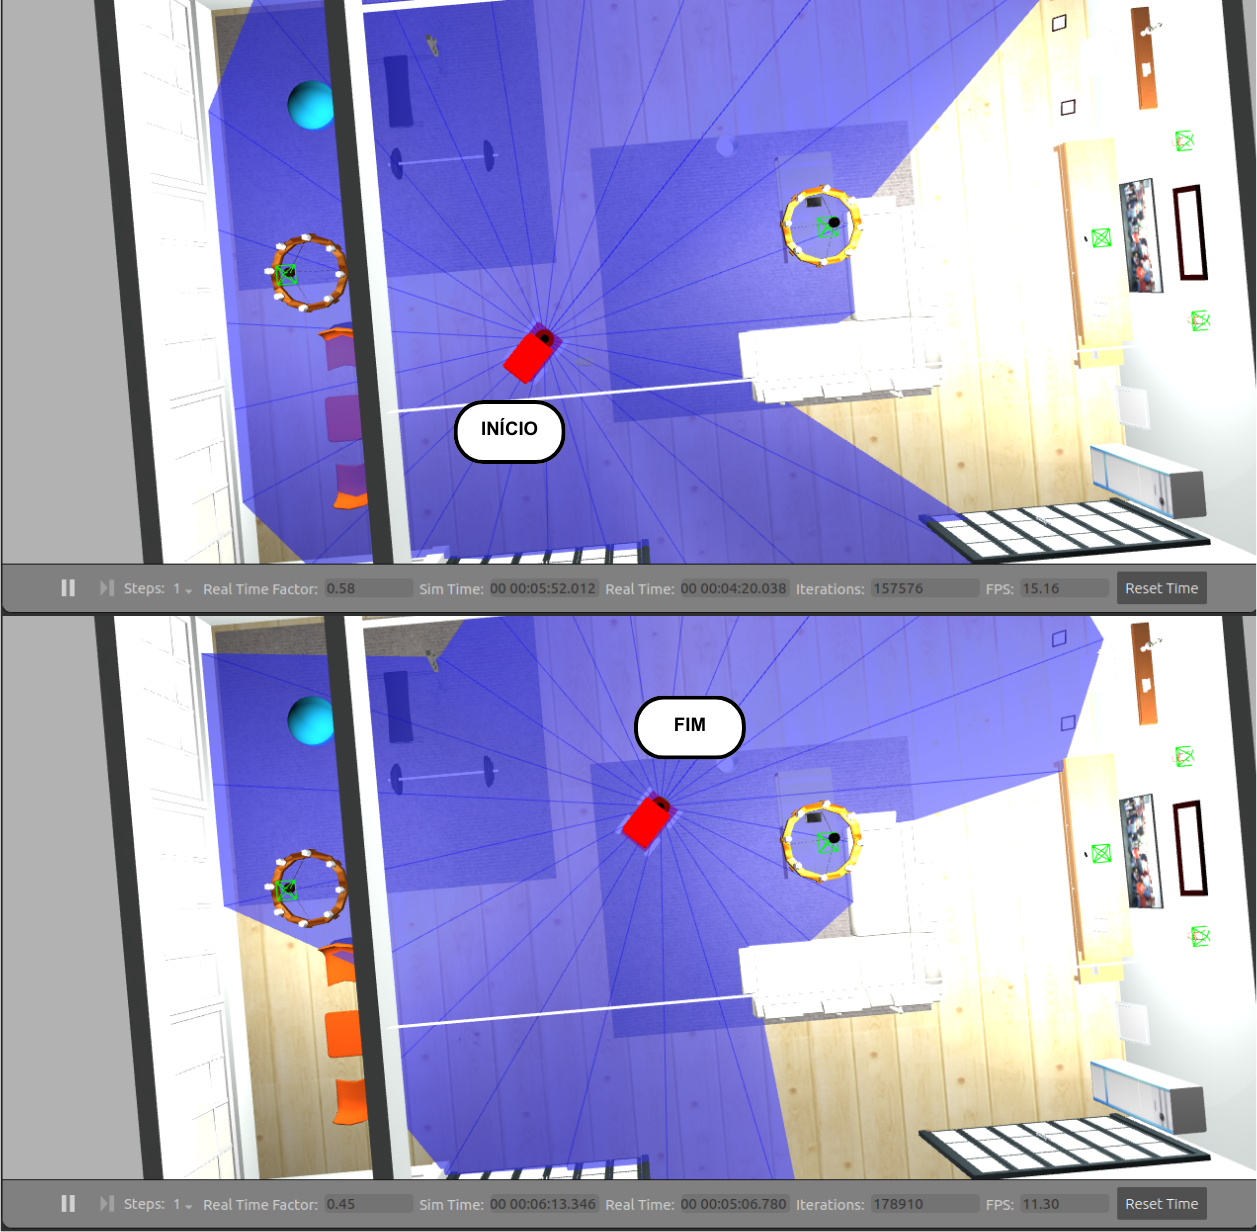
\includegraphics[scale=0.5]{ct03_4.png}
    \caption*{Fonte: Autora (2023).}
    \label{fig:ct03_4}
\end{figure}

\begin{figure}[H]
    \centering
    \caption{Captura da quinta repetição CT03}
    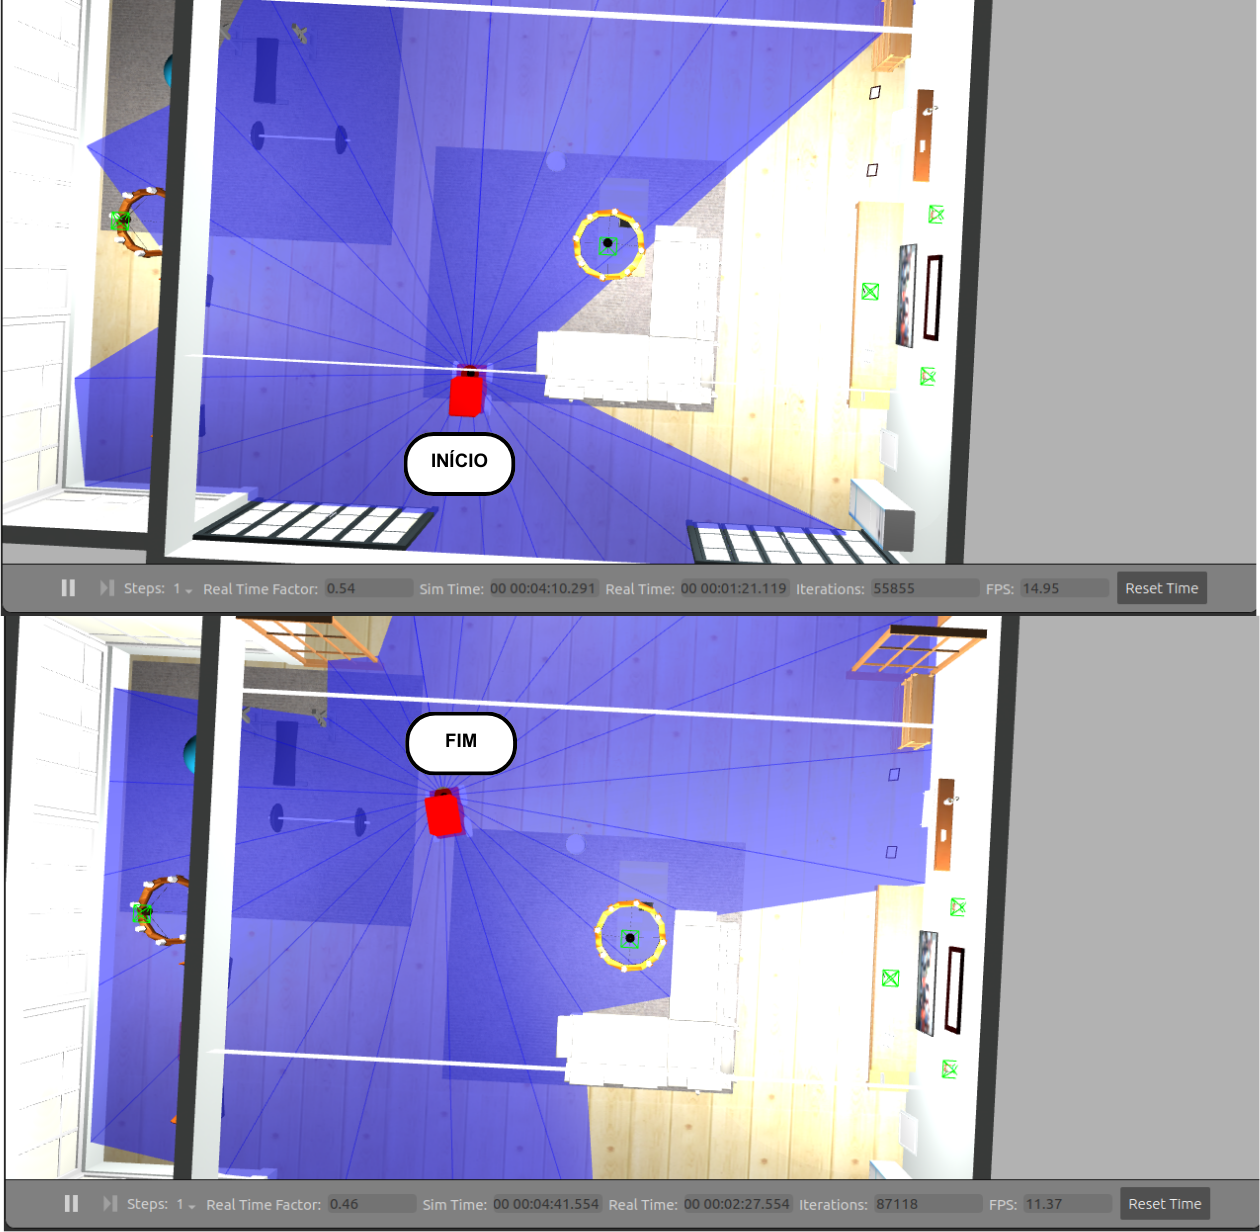
\includegraphics[scale=0.5]{ct03_5.png}
    \caption*{Fonte: Autora (2023).}
    \label{fig:ct03_5}
\end{figure}

\section{Caso de Teste CT04 Referente a RNFS02}
O caso de teste CT04 teve o objetivo de identificar se a velocidade do robô é segura para as pessoas e propriedades ao redor. O caso de teste foi repetido cinco vezes com o robô em lugares distintos no ambiente. Todos os cinco testes foram bem sucedidos. Todos os resultados podem ser visualizados na Tabela~\ref{tab:acertosct04}. Além disso, a seguir podem ser encontradas as capturas para cada repetição (Figura~\ref{fig:ct04_1}, Figura~\ref{fig:ct04_2}, Figura~\ref{fig:ct04_3}, Figura~\ref{fig:ct04_4}, Figura~\ref{fig:ct04_5}).


\begin{table}[H]
\centering
\caption{Resultados das repetições CT04}
\label{tab:acertosct04}
\resizebox{\textwidth}{!}{%
\begin{tabular}{l|c}
                              & \multicolumn{1}{l}{\textbf{Resultados CT04}} \\ \hline
\textbf{Teste 1}              & Bem-sucedido                                 \\
\textbf{Teste 2}              & Bem-sucedido                                 \\
\textbf{Teste 3}              & Bem-sucedido                                 \\
\textbf{Teste 4}              & Bem-sucedido                                 \\
\textbf{Teste 5}              & Bem-sucedido                                 \\
\textbf{Total de acertos (\%)} & \textbf{100}                                  \\ \hline
\end{tabular}%
}
\caption*{Fonte: Autora (2023).}
\end{table}

\begin{figure}[H]
    \centering
    \caption{Captura da primeira repetição CT04}
    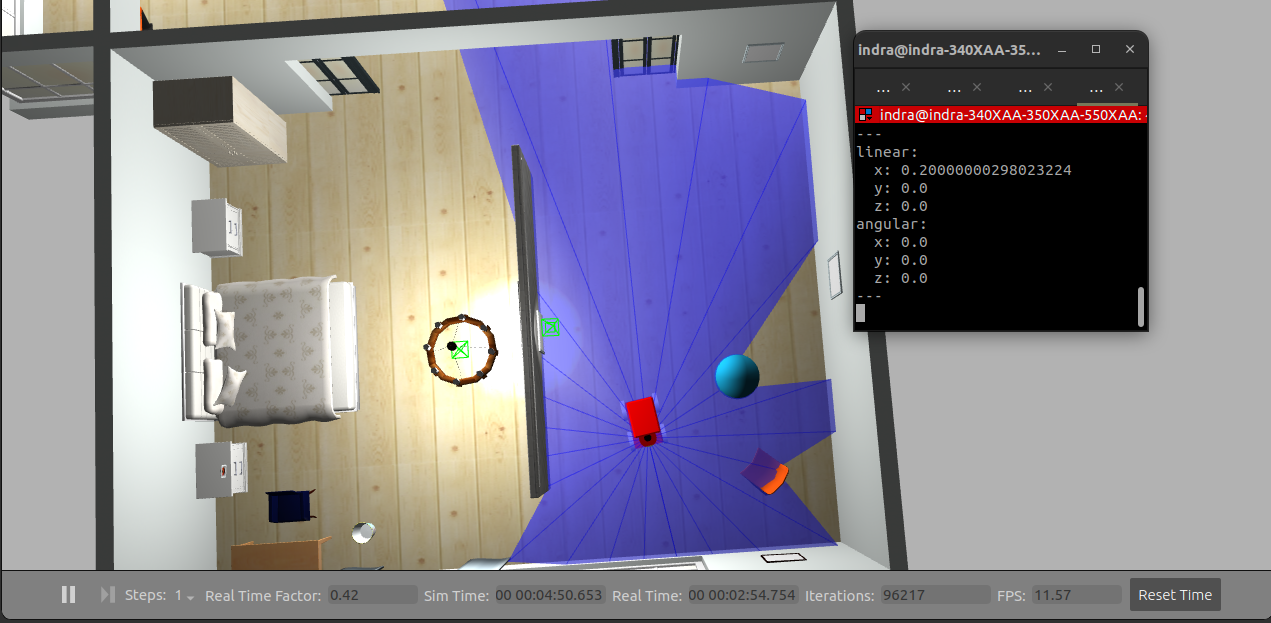
\includegraphics[scale=0.35]{ct04_1.png}
    \caption*{Fonte: Autora (2023).}
    \label{fig:ct04_1}
\end{figure}


\begin{figure}[H]
    \centering
    \caption{Captura da segunda repetição CT04}
    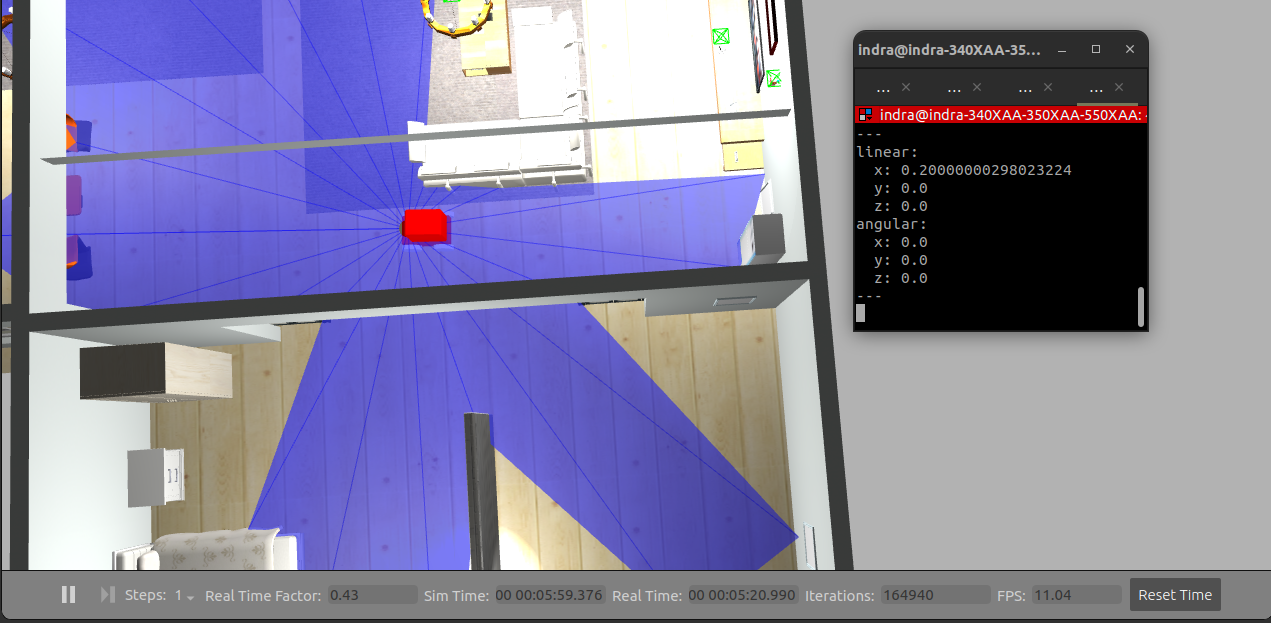
\includegraphics[scale=0.35]{ct04_2.png}
    \caption*{Fonte: Autora (2023).}
    \label{fig:ct04_2}
\end{figure}

\begin{figure}[H]
    \centering
    \caption{Captura da terceira repetição CT04}
    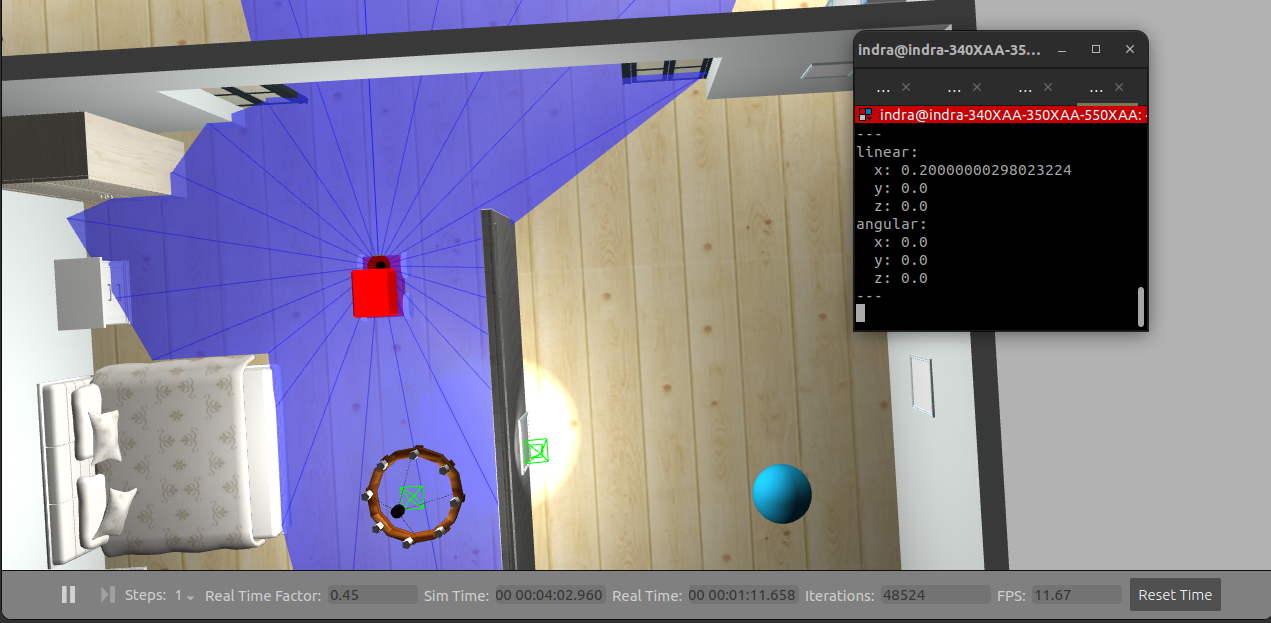
\includegraphics[scale=0.35]{ct04_3.png}
    \caption*{Fonte: Autora (2023).}
    \label{fig:ct04_3}
\end{figure}

\begin{figure}[H]
    \centering
    \caption{Captura da quarta repetição CT04}
    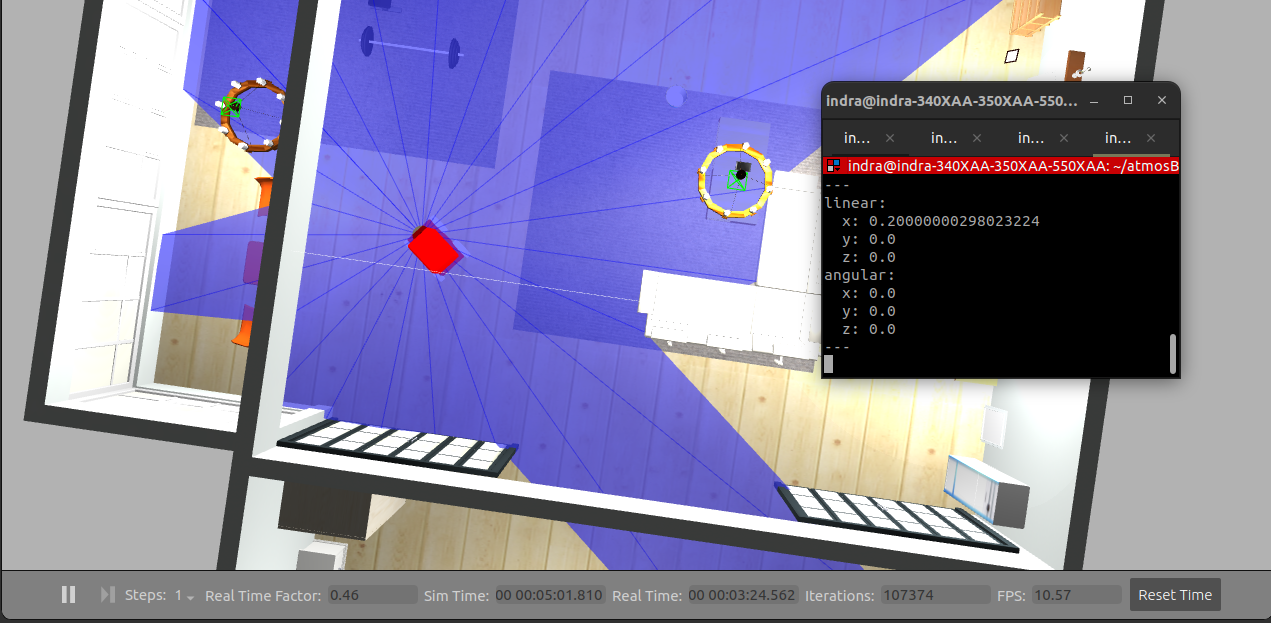
\includegraphics[scale=0.35]{ct04_4.png}
    \caption*{Fonte: Autora (2023).}
    \label{fig:ct04_4}
\end{figure}

\begin{figure}[H]
    \centering
    \caption{Captura da quinta repetição CT04}
    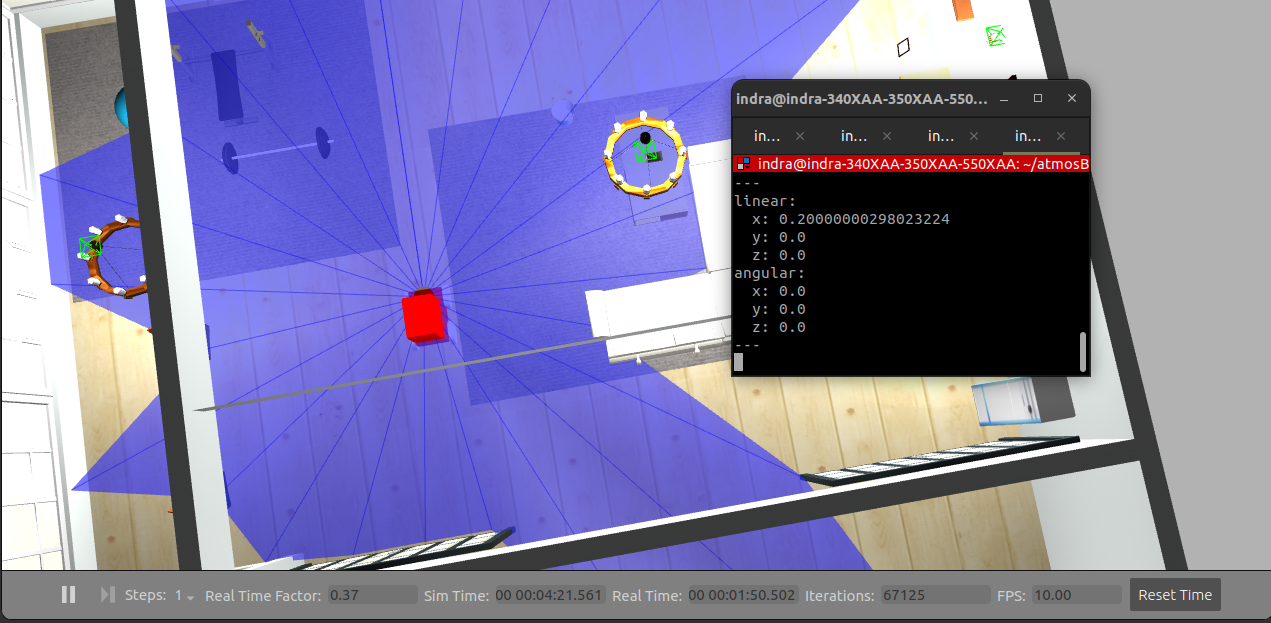
\includegraphics[scale=0.35]{ct04_5.png}
    \caption*{Fonte: Autora (2023).}
    \label{fig:ct04_5}
\end{figure}

\newpage

\section{Caso de Teste CT05 Referente a RNFA01}
O caso de teste CT05 visou validar se o ambiente simulado comportava a mudança de posição dos objetos e móveis ao longo da simulação. O caso de teste foi repetido cinco vezes com o robô em lugares distintos no ambiente. Todos os cinco testes foram bem sucedidos. Todos os resultados podem ser visualizados na Tabela~\ref{tab:acertosct05}. Além disso, a seguir podem ser encontradas as capturas para cada repetição (Figura~\ref{fig:ct05_1}, Figura~\ref{fig:ct05_2}, Figura~\ref{fig:ct05_3}, Figura~\ref{fig:ct05_4}, Figura~\ref{fig:ct05_5}).


\begin{table}[H]
\centering
\caption{Resultados das repetições CT05}
\label{tab:acertosct05}
\resizebox{\textwidth}{!}{%
\begin{tabular}{l|c}
                              & \multicolumn{1}{l}{\textbf{Resultados CT05}} \\ \hline
\textbf{Teste 1}              & Bem-sucedido                                 \\
\textbf{Teste 2}              & Bem-sucedido                                 \\
\textbf{Teste 3}              & Bem-sucedido                                 \\
\textbf{Teste 4}              & Bem-sucedido                                 \\
\textbf{Teste 5}              & Bem-sucedido                                 \\
\textbf{Total de acertos (\%)} & \textbf{100}                                  \\ \hline
\end{tabular}%
}
\caption*{Fonte: Autora (2023).}
\end{table}

\begin{figure}[H]
    \centering
    \caption{Captura da primeira repetição CT05}
    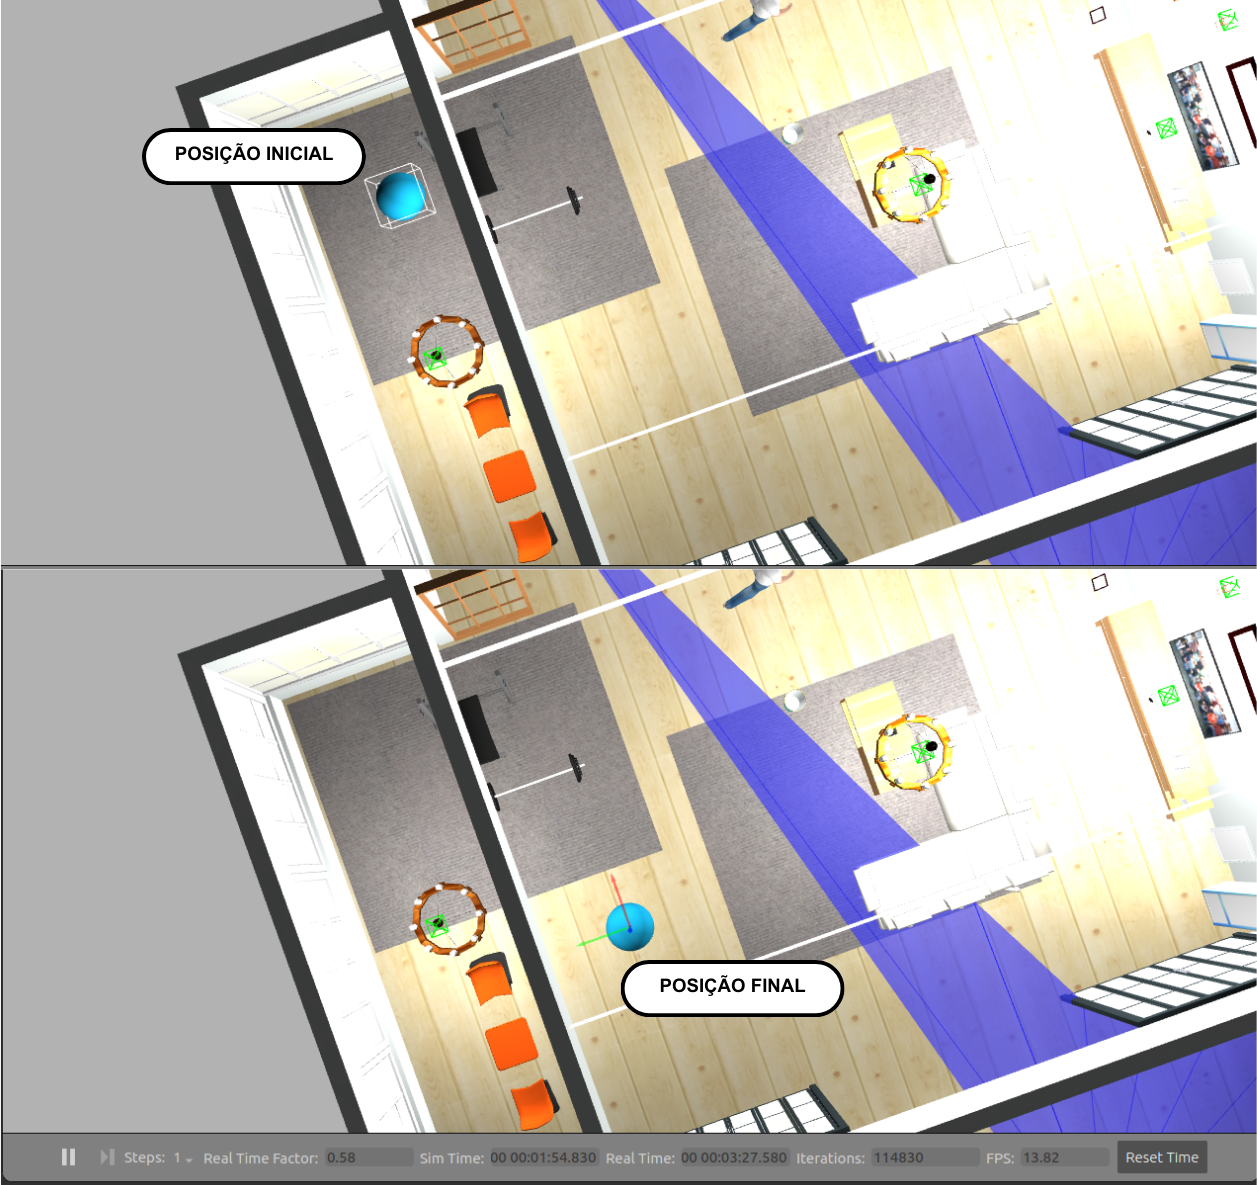
\includegraphics[scale=0.5]{ct05_1.png}
    \caption*{Fonte: Autora (2023).}
    \label{fig:ct05_1}
\end{figure}

\begin{figure}[H]
    \centering
    \caption{Captura da segunda repetição CT04}
    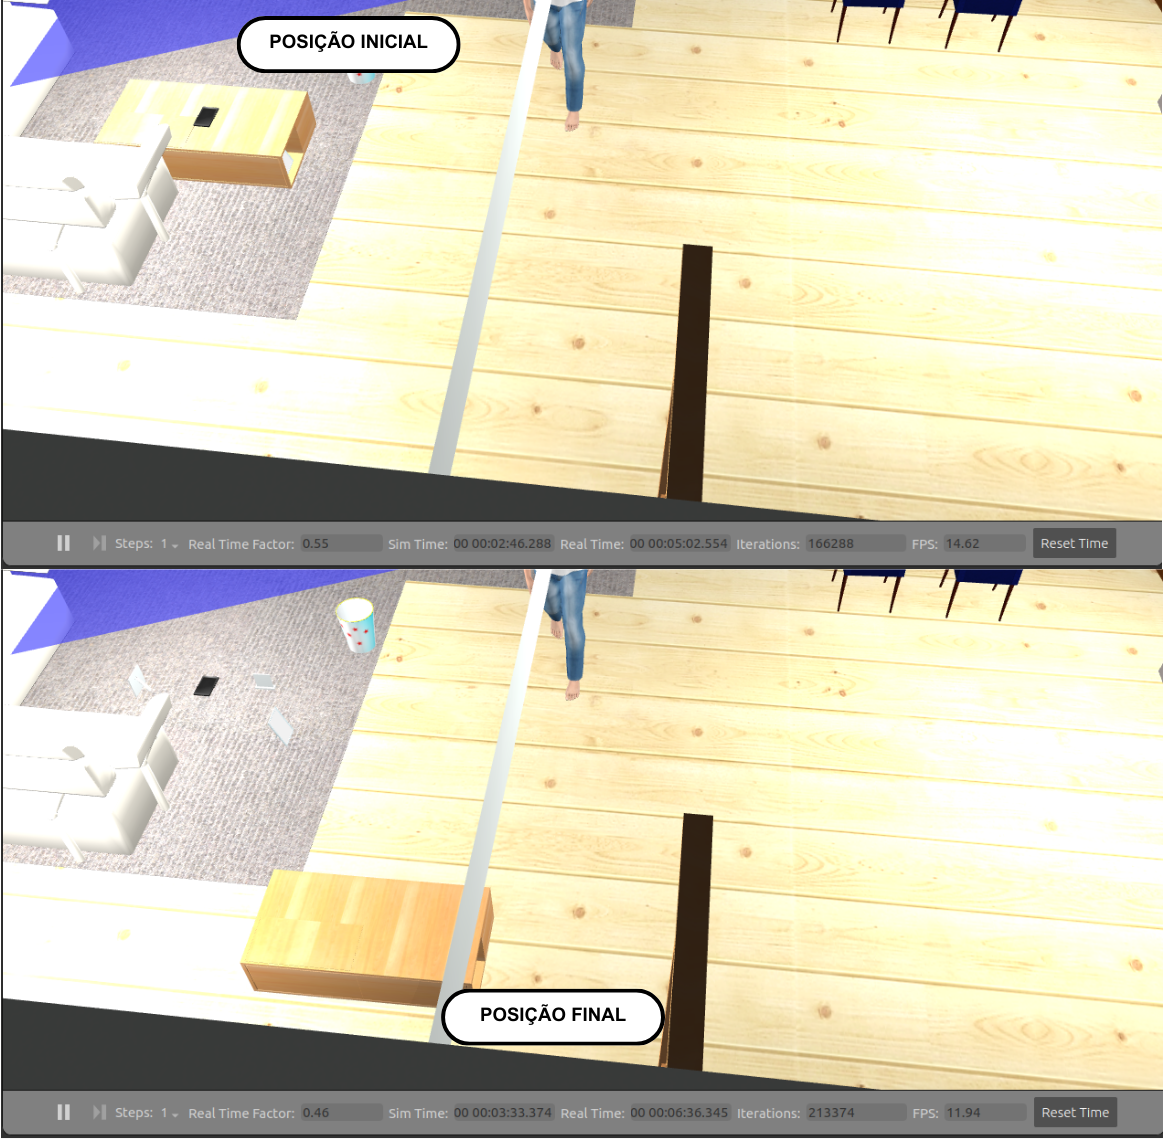
\includegraphics[scale=0.5]{ct05_2.png}
    \caption*{Fonte: Autora (2023).}
    \label{fig:ct05_2}
\end{figure}

\begin{figure}[H]
    \centering
    \caption{Captura da terceira repetição CT04}
    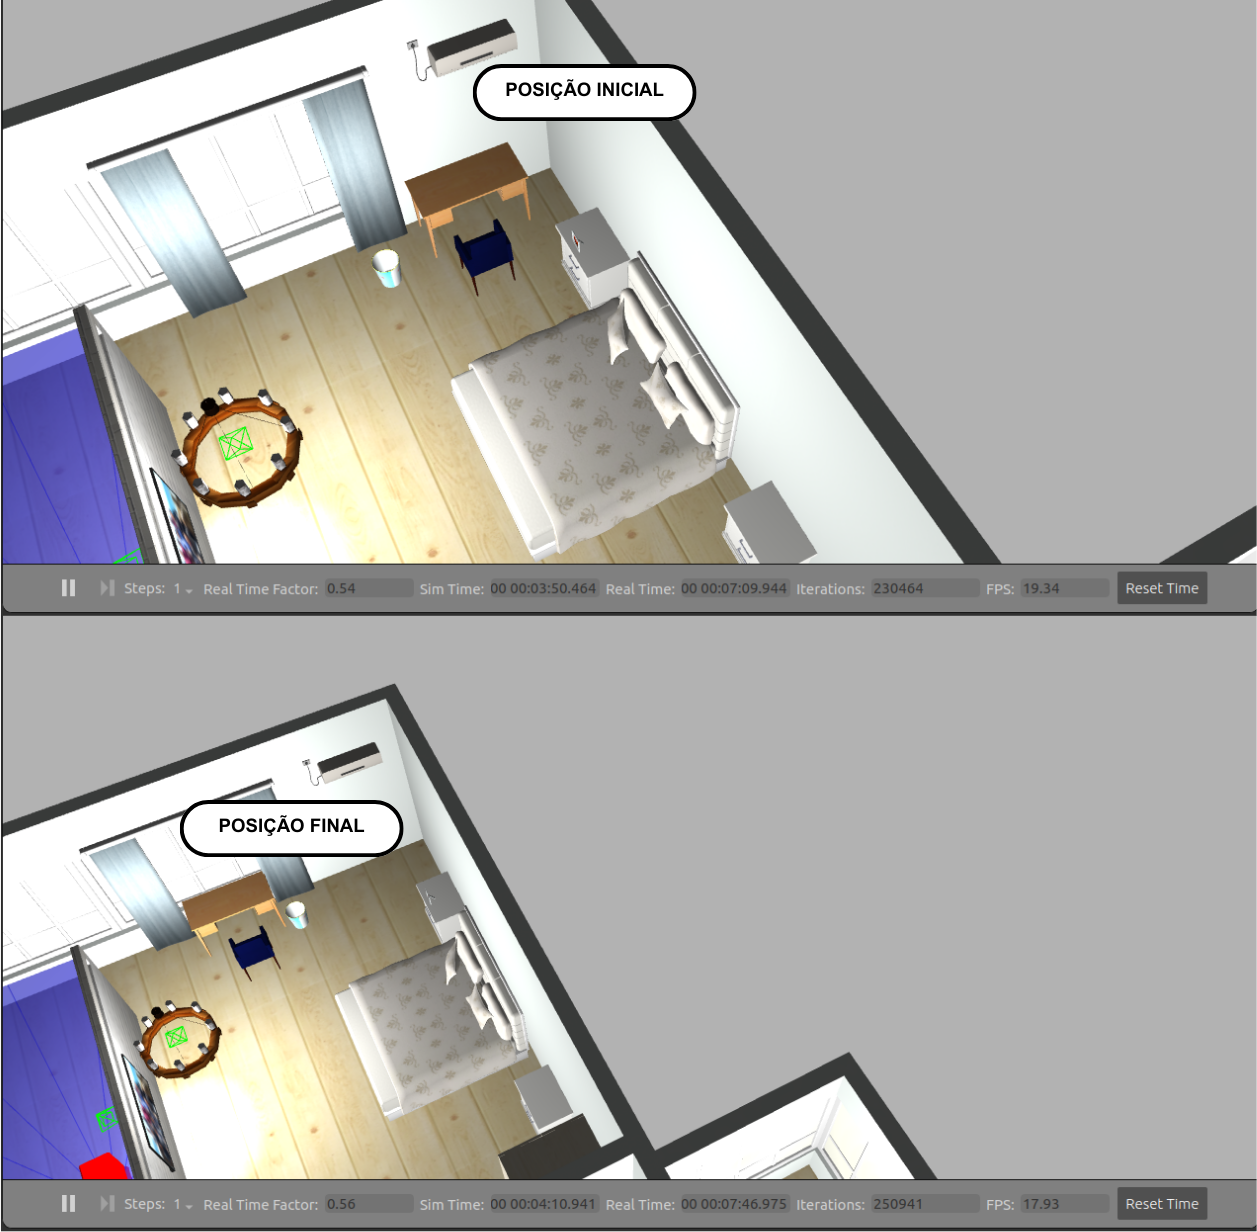
\includegraphics[scale=0.5]{ct05_3.png}
    \caption*{Fonte: Autora (2023).}
    \label{fig:ct05_3}
\end{figure}

\begin{figure}[H]
    \centering
    \caption{Captura da quarta repetição CT04}
    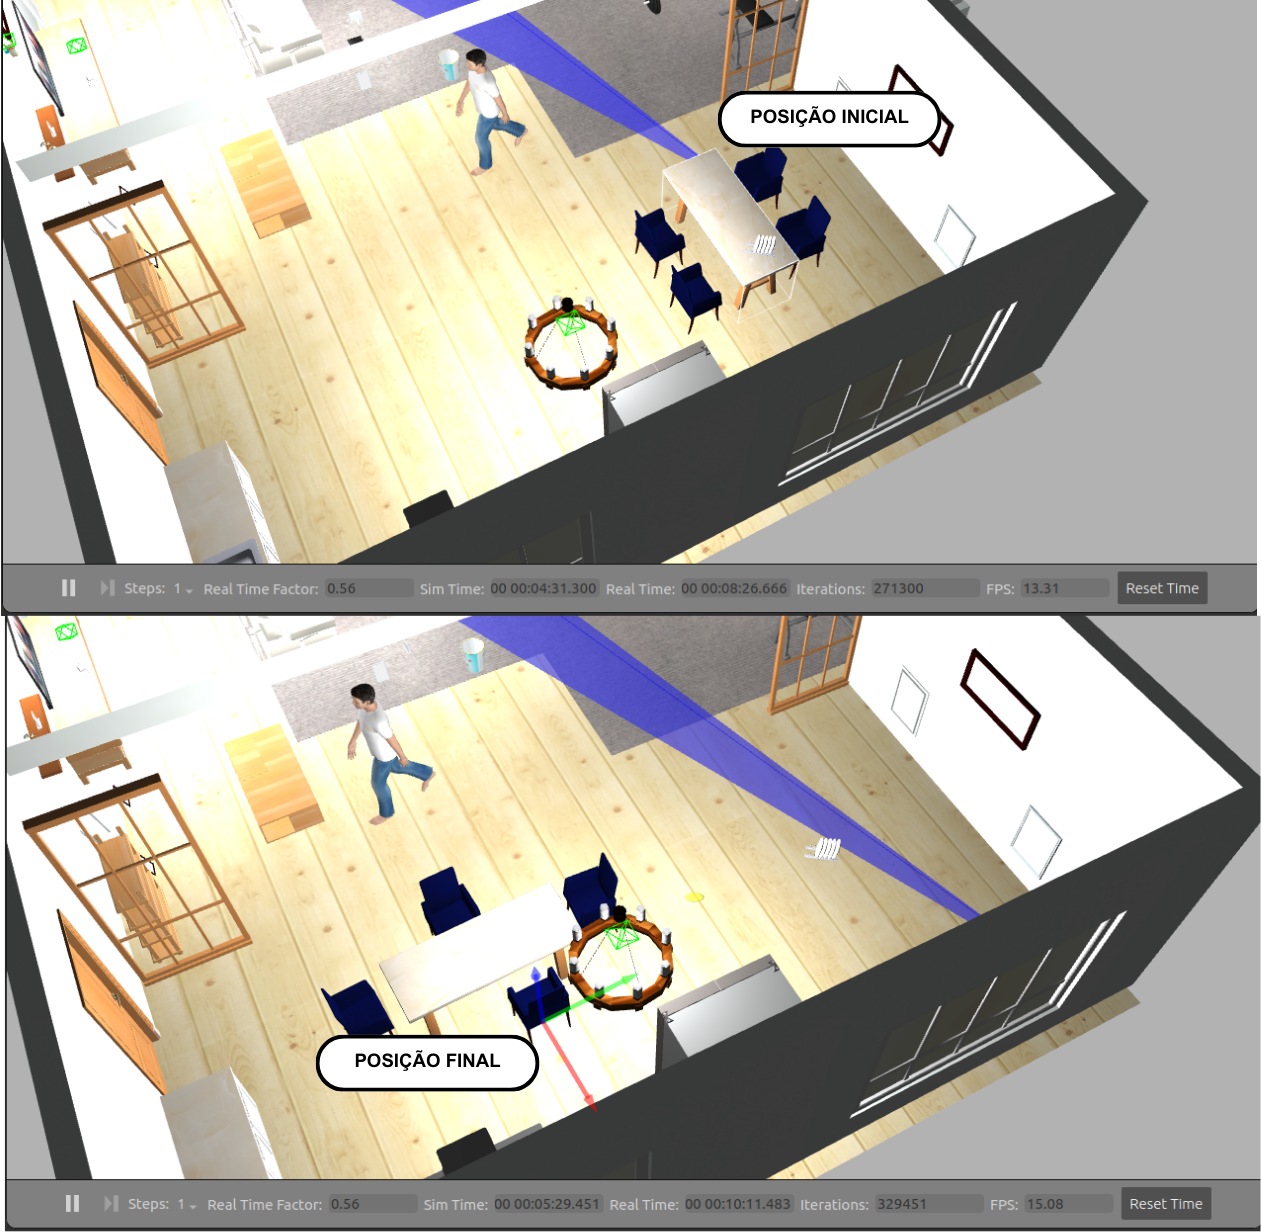
\includegraphics[scale=0.5]{ct05_4.png}
    \caption*{Fonte: Autora (2023).}
    \label{fig:ct05_4}
\end{figure}

\begin{figure}[H]
    \centering
    \caption{Captura da quinta repetição CT04}
    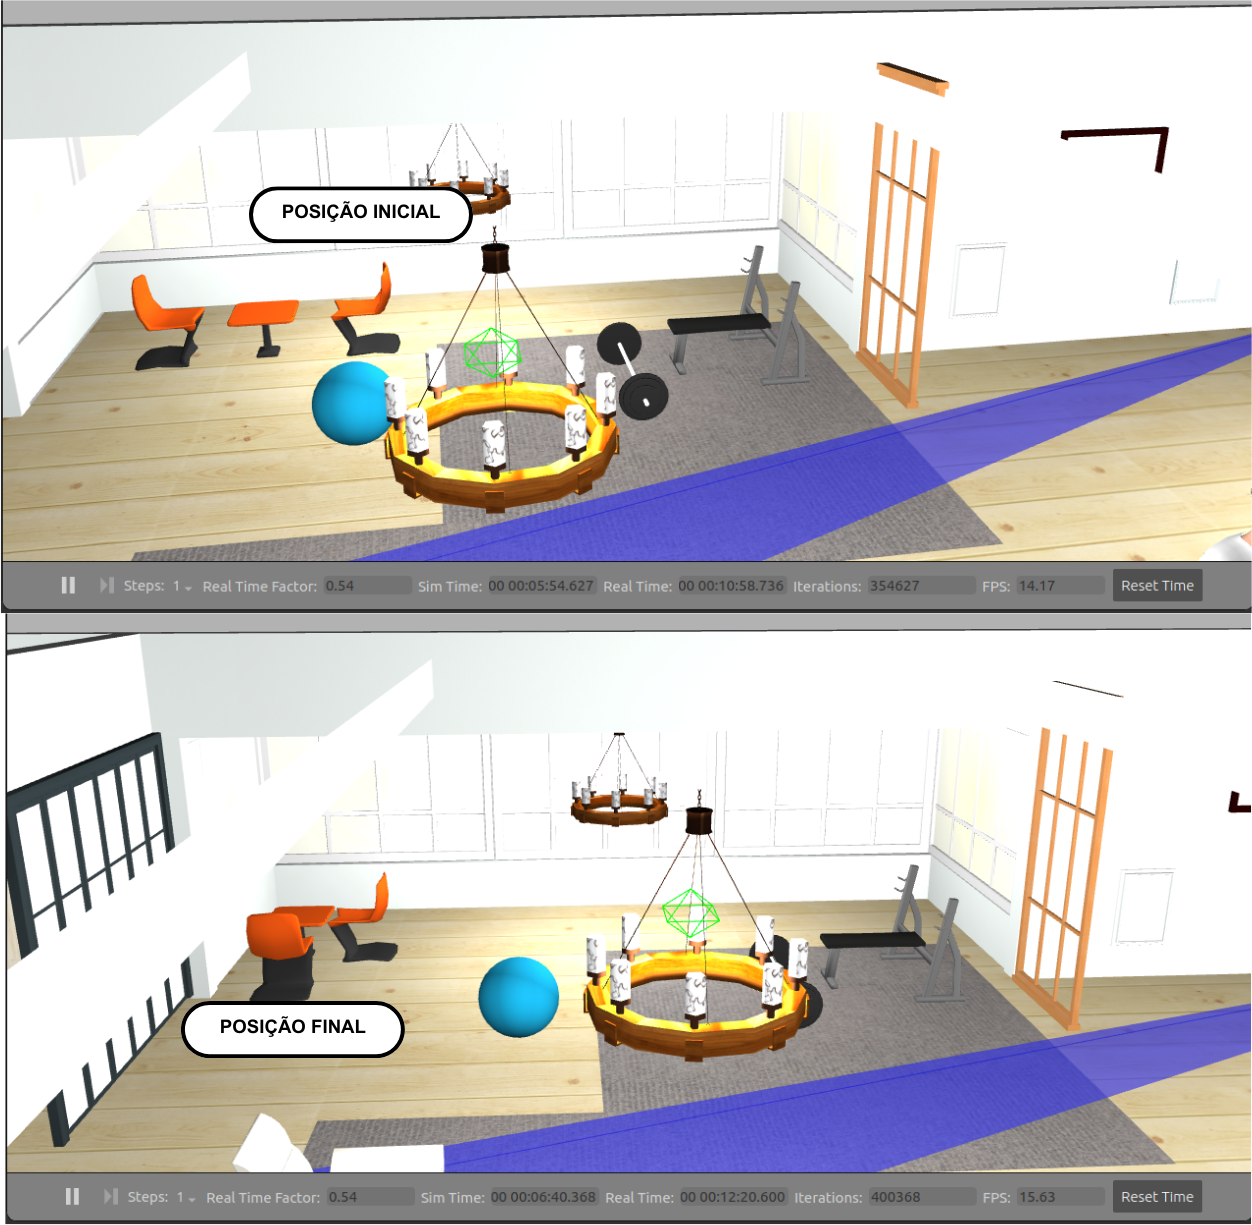
\includegraphics[scale=0.5]{ct05_5.png}
    \caption*{Fonte: Autora (2023).}
    \label{fig:ct05_5}
\end{figure}

\section{Caso de Teste CT06 Referente a RNFA03}
O caso de teste CT06 teve o objetivo de identificar se a simulação apresenta um ambiente semelhante a um domicílio comum. Na Figura~\ref{fig:ct06}, pode ser encontrada a captura do teste.

\begin{figure}[H]
    \centering
    \caption{Captura do teste CT06}
    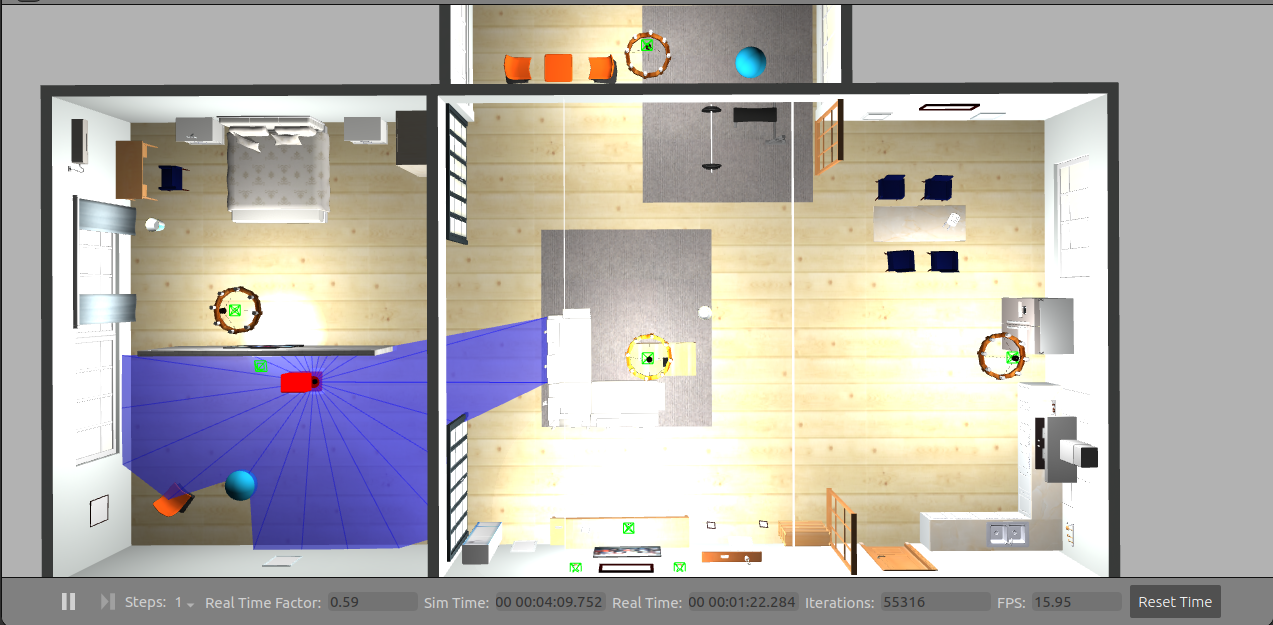
\includegraphics[scale=0.35]{ct06.png}
    \caption*{Fonte: Autora (2023).}
    \label{fig:ct06}
\end{figure}

\section{Caso de Teste CT07 Referente a RNFA04}
O caso de teste CT07 teve o objetivo de identificar o tamanho do domicílio apresentado na simulação. Na Figura~\ref{fig:ct07}, pode ser encontrada a captura do teste.

\begin{figure}[H]
    \centering
    \caption{Captura do teste CT07}
    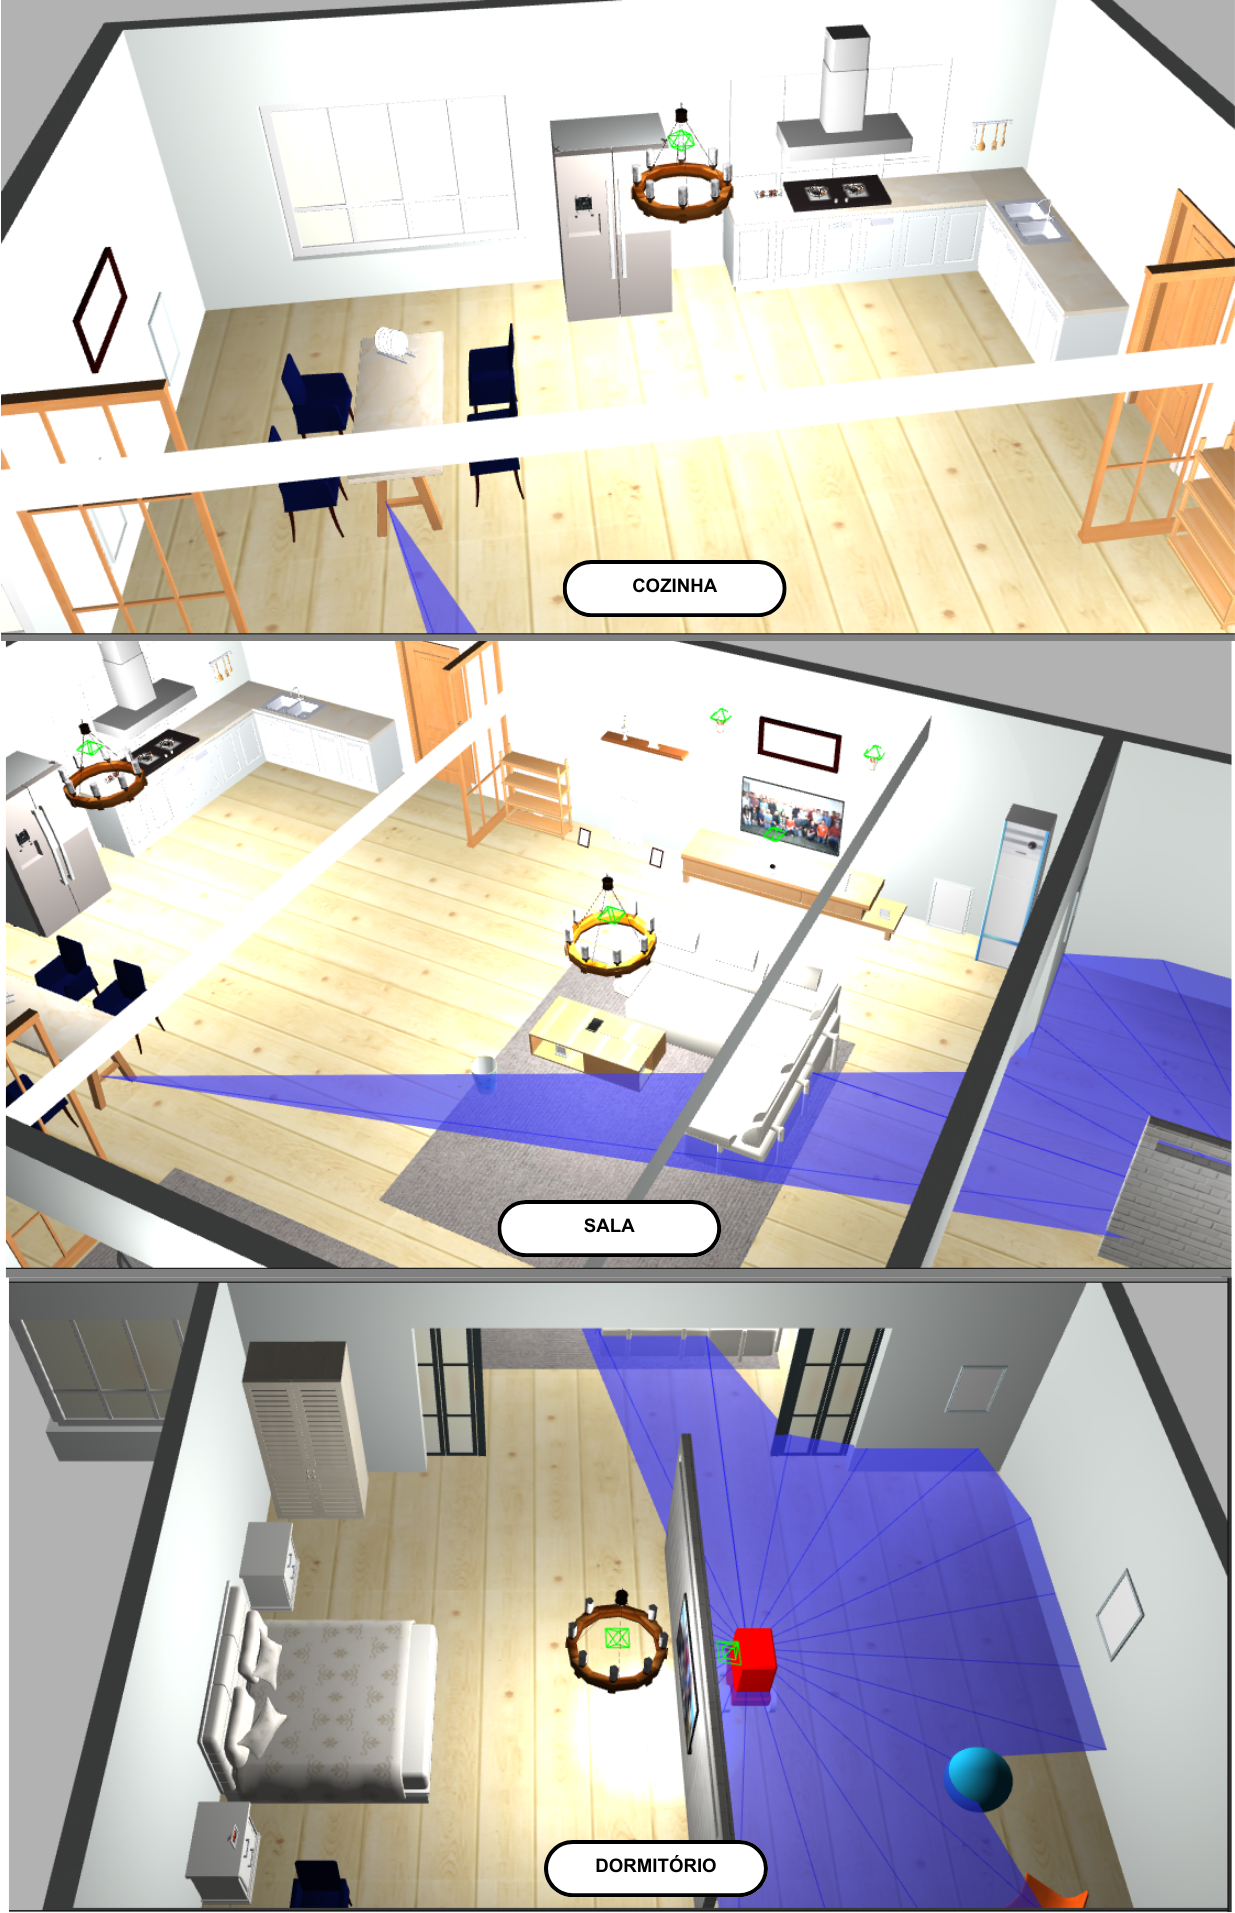
\includegraphics[scale=0.45]{ct07.png}
    \caption*{Fonte: Autora (2023).}
    \label{fig:ct07}
\end{figure}

\section{Caso de Teste CT08 Referente a RNFA05}
O caso de teste CT08 visou identificar o acesso entre os espaços do ambiente simulado. Na Figura~\ref{fig:ct08}, pode ser encontrada a captura do teste.

\begin{figure}[H]
    \centering
    \caption{Captura do teste CT08}
    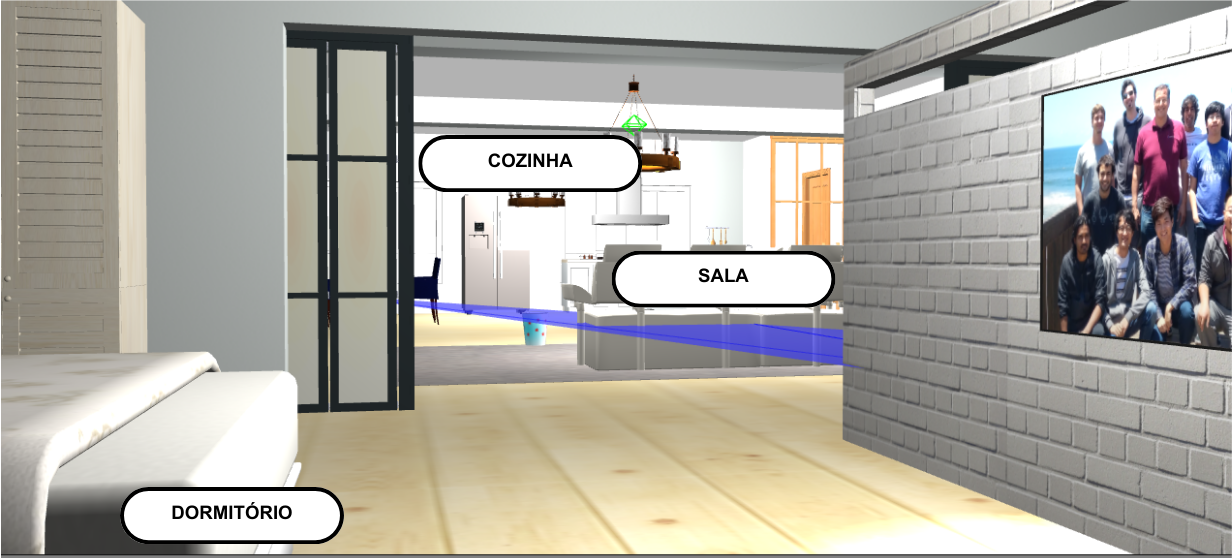
\includegraphics[scale=0.5]{ct08.png}
    \caption*{Fonte: Autora (2023).}
    \label{fig:ct08}
\end{figure}